%%
%% This is file `sample-sigconf.tex',
%% generated with the docstrip utility.
%%
%% The original source files were:
%%
%% samples.dtx  (with options: `sigconf')
%% 
%% IMPORTANT NOTICE:
%% 
%% For the copyright see the source file.
%% 
%% Any modified versions of this file must be renamed
%% with new filenames distinct from sample-sigconf.tex.
%% 
%% For distribution of the original source see the terms
%% for copying and modification in the file samples.dtx.
%% 
%% This generated file may be distributed as long as the
%% original source files, as listed above, are part of the
%% same distribution. (The sources need not necessarily be
%% in the same archive or directory.)
%%
%%
%% Commands for TeXCount
%TC:macro \cite [option:text,text]
%TC:macro \citep [option:text,text]
%TC:macro \citet [option:text,text]
%TC:envir table 0 1
%TC:envir table* 0 1
%TC:envir tabular [ignore] word
%TC:envir displaymath 0 word
%TC:envir math 0 word
%TC:envir comment 0 0
%%
%%
%% The first command in your LaTeX source must be the \documentclass command.

%\documentclass[sigconf]{acmart}
%\documentclass[sigconf,screen]{acmart}

\PassOptionsToPackage{table,xcdraw}{xcolor}

\documentclass[sigconf,review,anonymous]{acmart}
\acmConference[ESEC/FSE 2023]{The 31st ACM Joint European Software Engineering Conference and Symposium on the Foundations of Software Engineering}{11 - 17 November, 2023}{San Francisco, USA}

%%
%% \BibTeX command to typeset BibTeX logo in the docs
\AtBeginDocument{%
  \providecommand\BibTeX{{%
    Bib\TeX}}}

%\usepackage{amsmath,amssymb,amsfonts}
%\usepackage{algorithmic}
\usepackage{graphicx}
\usepackage{textcomp}
%\usepackage{xcolor}

\usepackage[table]{xcolor}

\def\BibTeX{{\rm B\kern-.05em{\sc i\kern-.025em b}\kern-.08em
    T\kern-.1667em\lower.7ex\hbox{E}\kern-.125emX}}

%\usepackage{cite}
\usepackage{booktabs}   %% For formal tables:
                        %% http://ctan.org/pkg/booktabs
%\usepackage{subcaption} %% For complex figures with subfigures/subcaptions
                        %% http://ctan.org/pkg/subcaption
\usepackage{array}
%\usepackage{amsmath,amsfonts}
%\usepackage{amssymb}
%\usepackage{algorithm}
%\usepackage[noend]{algpseudocode}
%\usepackage{algorithmic}
%\usepackage{graphicx}
%\usepackage{textcomp}
\usepackage{float}
\usepackage{listings}
\usepackage{xspace}
\usepackage{multirow}
%\usepackage{amsthm}
%\usepackage[skins]{tcolorbox}

\newtheorem{definition}{Definition}
\usepackage{balance}

\usepackage[skins]{tcolorbox}


\usepackage{xcolor,pifont}
\newcommand*\colourcheck[1]{%
	\expandafter\newcommand\csname #1check\endcsname{\textcolor{#1}{\ding{52}}}%
}
\colourcheck{blue}
\colourcheck{green}
\colourcheck{red}

\newtcolorbox{myframe}[2][]{%
  enhanced,colback=white,colframe=black,coltitle=black,
  sharp corners,
  toprule=1.0pt,
  rightrule=0.3pt,
  leftrule=0pt,
  bottomrule=0pt,
  fonttitle=\itshape\scshape\large,
  left=0pt,right=5pt,top=5pt,bottom=3pt,
  attach boxed title to top right={yshift=-0.3\baselineskip-0.4pt,xshift=-5mm},
  boxed title style={tile,size=minimal,left=0.2mm,right=0.5mm,
    colback=white,before upper=\strut},
  title=#2,#1
}

\newcommand{\tool}{\textsc{CDFix}\xspace}

\newtheorem{Definition}{Definition}
\newtheorem{Claim}{Claim}
\newtheorem{Lemma}{Lemma}
\newtheorem{Theorem}{Theorem}

\newcolumntype{L}[1]{>{\raggedright\arraybackslash}p{#1}}
\newtheorem{observation}{Observation}
\newtheorem{property}{Property}
\newcommand{\code}[1]{{\footnotesize\texttt{#1}}}
\usepackage{amsthm}
 \definecolor{dkgreen}{rgb}{0,0.6,0}
\definecolor{gray}{rgb}{0.5,0.5,0.5}
\definecolor{mauve}{rgb}{0.58,0,0.82}
\lstset{frame=tb,
  language=Java,
  aboveskip=3mm,
  belowskip=3mm,
  showstringspaces=false,
  columns=flexible,
  basicstyle={\small\ttfamily},
  numbers=left,
  numberstyle=\tiny\color{gray},
  keywordstyle=\color{blue},
  commentstyle=\color{dkgreen},
  stringstyle=\color{mauve},
  breaklines=true,
  breakatwhitespace=true,
  tabsize=4
}


%% Rights management information.  This information is sent to you
%% when you complete the rights form.  These commands have SAMPLE
%% values in them; it is your responsibility as an author to replace
%% the commands and values with those provided to you when you
%% complete the rights form.
%\setcopyright{acmcopyright}
%\copyrightyear{2018}
%\acmYear{2018}
%\acmDOI{XXXXXXX.XXXXXXX}

%% These commands are for a PROCEEDINGS abstract or paper.
%\acmConference[Conference acronym 'XX]{Make sure to enter the correct
%  conference title from your rights confirmation emai}{June 03--05,
%  2018}{Woodstock, NY}
%\acmPrice{15.00}
%\acmISBN{978-1-4503-XXXX-X/18/06}


%%% If you see 'ACMUNKNOWN' in the 'setcopyright' statement below,
%%% please first submit your publishing-rights agreement with ACM (follow link on submission page).
%%% Then please update our instructions page and copy-and-paste the NEW commands into your article.
%%% Please contact us in case of questions; allow up to 10 min for the system to propagate the information.
%%%

%%% The following is specific to ESEC/FSE '22 and the paper
%%% 'UTANGO: Untangling Commits with Context-Aware, Graph-Based, Code Change Clustering Learning Model'
%%% by Yi Li, Shaohua Wang, and Tien N. Nguyen.
%%%

%\setcopyright{acmcopyright}
%\acmPrice{15.00}
%\acmDOI{10.1145/3540250.3549171}
%\acmYear{2022}
%\copyrightyear{2022}
%\acmSubmissionID{fse22main-p1469-p}
%\acmISBN{978-1-4503-9413-0/22/11}
%\acmConference[ESEC/FSE '22]{Proceedings of the 30th ACM Joint European Software Engineering Conference and Symposium on the Foundations of Software Engineering}{November 14--18, 2022}{Singapore, Singapore}
%\acmBooktitle{Proceedings of the 30th ACM Joint European Software Engineering Conference and Symposium on the Foundations of Software Engineering (ESEC/FSE '22), November 14--18, 2022, Singapore, Singapore}

%\setcopyright{ACMUNKNOWN}
%\acmPrice{15.00}
%\acmDOI{10.1145/3540250.3549137}
%\acmYear{2022}
%\copyrightyear{2022}
%\acmSubmissionID{fse22main-p639-p}
%\acmISBN{978-1-4503-9413-0/22/11}
%\acmConference[ESEC/FSE '22]{Proceedings of the 30th ACM Joint European Software Engineering Conference and Symposium on the Foundations of Software Engineering}{November 14--18, 2022}{Singapore, Singapore}
%\acmBooktitle{Proceedings of the 30th ACM Joint European Software Engineering Conference and Symposium on the Foundations of Software Engineering (ESEC/FSE '22), November 14--18, 2022, Singapore, Singapore}

%\copyrightyear{2022}
%\acmYear{2022}
%\setcopyright{acmcopyright}
%\acmConference[ESEC/FSE '22]{Proceedings of the 30th ACM Joint European Software Engineering Conference and Symposium on the Foundations of Software Engineering}{November 14--18, 2022}{Singapore, Singapore}
%\acmBooktitle{Proceedings of the 30th ACM Joint European Software Engineering Conference and Symposium on the Foundations of Software Engineering (ESEC/FSE '22), November 14--18, 2022, Singapore, Singapore}
%\acmPrice{15.00}
%\acmDOI{10.1145/3540250.3549137}
%\acmISBN{978-1-4503-9413-0/22/11}


%%
%% Submission ID.
%% Use this when submitting an article to a sponsored event. You'll
%% receive a unique submission ID from the organizers
%% of the event, and this ID should be used as the parameter to this command.
%%\acmSubmissionID{123-A56-BU3}

%%
%% For managing citations, it is recommended to use bibliography
%% files in BibTeX format.
%%
%% You can then either use BibTeX with the ACM-Reference-Format style,
%% or BibLaTeX with the acmnumeric or acmauthoryear sytles, that include
%% support for advanced citation of software artefact from the
%% biblatex-software package, also separately available on CTAN.
%%
%% Look at the sample-*-biblatex.tex files for templates showcasing
%% the biblatex styles.
%%

%%
%% The majority of ACM publications use numbered citations and
%% references.  The command \citestyle{authoryear} switches to the
%% "author year" style.
%%
%% If you are preparing content for an event
%% sponsored by ACM SIGGRAPH, you must use the "author year" style of
%% citations and references.
%% Uncommenting
%% the next command will enable that style.
%%\citestyle{acmauthoryear}



%%
%% end of the preamble, start of the body of the document source.
\begin{document}

%%
%% The "title" command has an optional parameter,
%% allowing the author to define a "short title" to be used in page headers.
%\title{The Name of the Title Is Hope}

%\title[{\tool}: Context-aware Dual-Task Learning for Automated Program Repair]{{\tool}: Context-aware Dual-Task Learning for Automated Program Repair}

\title[Dual-Task of Context Learning and Code-Transformation Learning to Improve Automated Program Repair]{Dual-Task of Context Learning and Code-Transformation Learning to Improve Automated Program Repair}

\setcopyright{none}

\settopmatter{printacmref=false, printfolios=false}

\renewcommand\footnotetextcopyrightpermission[1]{} % removes footnote with conference information in first column

%%
%% The "author" command and its associated commands are used to define
%% the authors and their affiliations.
%% Of note is the shared affiliation of the first two authors, and the
%% "authornote" and "authornotemark" commands
%% used to denote shared contribution to the research.

%\author{Ben Trovato}
%\authornote{Both authors contributed equally to this research.}
%\email{trovato@corporation.com}
%\orcid{1234-5678-9012}
%\author{G.K.M. Tobin}
%\authornotemark[1]
%\email{webmaster@marysville-ohio.com}
%\affiliation{%
%  \institution{Institute for Clarity in Documentation}
%  \streetaddress{P.O. Box 1212}
%  \city{Dublin}
%  \state{Ohio}
%  \country{USA}
%  \postcode{43017-6221}
%}

%\author{Lars Th{\o}rv{\"a}ld}
%\affiliation{%
%  \institution{The Th{\o}rv{\"a}ld Group}
%  \streetaddress{1 Th{\o}rv{\"a}ld Circle}
%  \city{Hekla}
%  \country{Iceland}}
%\email{larst@affiliation.org}

%\author{Valerie B\'eranger}
%\affiliation{%
%  \institution{Inria Paris-Rocquencourt}
%  \city{Rocquencourt}
%  \country{France}
%}

%\author{Aparna Patel}
%\affiliation{%
% \institution{Rajiv Gandhi University}
% \streetaddress{Rono-Hills}
% \city{Doimukh}
% \state{Arunachal Pradesh}
% \country{India}}

%\author{Huifen Chan}
%\affiliation{%
%  \institution{Tsinghua University}
%  \streetaddress{30 Shuangqing Rd}
%  \city{Haidian Qu}
%  \state{Beijing Shi}
%  \country{China}}

%\author{Charles Palmer}
%\affiliation{%
%  \institution{Palmer Research Laboratories}
%  \streetaddress{8600 Datapoint Drive}
%  \city{San Antonio}
%  \state{Texas}
%  \country{USA}
%  \postcode{78229}}
%\email{cpalmer@prl.com}

%\author{John Smith}
%\affiliation{%
%  \institution{The Th{\o}rv{\"a}ld Group}
%  \streetaddress{1 Th{\o}rv{\"a}ld Circle}
%  \city{Hekla}
%  \country{Iceland}}
%\email{jsmith@affiliation.org}

%\author{Julius P. Kumquat}
%\affiliation{%
%  \institution{The Kumquat Consortium}
%  \city{New York}
%  \country{USA}}
%\email{jpkumquat@consortium.net}

%\renewcommand{\shortauthors}{Yi Li, Shaohua Wang, and Tien N. Nguyen}


%%
%% By default, the full list of authors will be used in the page
%% headers. Often, this list is too long, and will overlap
%% other information printed in the page headers. This command allows
%% the author to define a more concise list
%% of authors' names for this purpose.

%\renewcommand{\shortauthors}{Trovato et al.}

%%
%% The abstract is a short summary of the work to be presented in the
%% article.


%Our empirical evaluation on a C\# dataset with 1,612 tangled commits
%shows that it achieves the accuracy of 28.6\%--462.5\%, relatively
%higher than the state-of-the-art approaches in clustering the changed
%code. We evaluated {\tool} in a Java dataset with +14k
%tangled commits. The result shows that it achieves 13.3\%--100.0\%
%relatively higher accuracy than the state-of-the-art~approaches.



%Exploring this duality provides useful constraints for {\tool} to
%learn derive CC fixing statements.

%DEAR and CURE in which we replaced their FL modules with our tool.
%exploit this duality. In a cross-stitch unit, the sharing of
%representations between \code{MethFL} and \code{StmtFL} is modeled by
%the learning a linear combination of the input features from two
%models.  The cross-stitch units

%%
%% The code below is generated by the tool at http://dl.acm.org/ccs.cfm.
%% Please copy and paste the code instead of the example below.
%%

\begin{abstract}
%Recent advances in deep learning (DL) have helped improve the
%performance of the DL-based Automated Program Repair (APR) approaches.
The bug-fixing code changes in Automated Program Repair (APR) often
depend on the code context. Despite successes, the state-of-the-art
Deep Learning (DL)-based APR approaches are still limited in {\em
  integrating context learning and code-transformation learning},
leading to their ineffectiveness in fixing {\em context-dependent
  bugs}. {\em Learning the correct context for a bug will help
  learning the correct code transformation for the bug fix, and vice
  versa}. In this work, we introduce {\bf \tool}, a context-aware
dual-task learning APR model, that explores the duality of the two
dedicated models to explicitly propagate the mutual impacts of {\em
  context learning} and {\em code transformation learning} onto one
another. We train two models simultaneously with soft-sharing
parameters via a cross-stitch unit for explicit propagation of impacts
to improve both tasks, leading to better APR accuracy.


%Moreover, in those approaches, the cascading architecture from a code
%context-learning model (CCL) to a code-transformation learning model
%(CTL) possibly leads to confounding inaccuracies.
%In this work, we introduce {\bf \tool}, a context-aware dual-task
%learning APR model, that explores the duality of those two dedicated
%models to explicitly propagate the mutual impacts of CCL and CTL onto
%one another. Instead of cascading CCL $\rightarrow$ CTL, we train them
%simultaneously with soft-sharing parameters via a cross-stitch unit
%for explicit propagation of impacts to improve both tasks, leading
%to better APR accuracy.

We conducted several experiments to evaluate {\tool} on three
different datasets: Defects4J~\cite{defects4j} (395 bugs),
Bugs.jar~\cite{saha2018bugs} (1,158 bugs), and
BigFix~\cite{yioopsla19} (+4.9M methods and 1.8M buggy ones).  We
compared {\tool} against several state-of-the-art DL-based APR
tools. Our results show that {\tool} can fix 16.7\%, 12.1\%, and
14.6\% more bugs than the best-performance DL-based baseline model
with only top-1 patches in Defects4J, Bugs.jar, and BigFix,
respectively. In Defects4J, it improves over the baselines
from 16.7\%--194.7\%. In Bugs.jar and BigFix, it fixes 26.4\% and
27.7\% of the total bugs that were missed by the best DL-based
baseline.

\end{abstract}

%\keywords{Code Completion, Code prediction, Neural Network}

\maketitle

\section{Introduction}

%Fixing software defects is one of the crucial maintenance
%activities. Thus,

%Detecting and fixing software defects is one of the most crucial
%activities in software development.
Researchers have developed the approaches to automate the
bug-fixing task. The approaches that help
developers automatically fix a software defect is
referred to as {\em automated program repair} (APR). The APR
approaches can be broadly classified in the following categories
based on their techniques:
%Researchers have proposed several approaches to help developers in
%automatically identifying and fixing the defects in programs. Such
%approaches are referred to as {\em automated program~repair}
%(APR). The APR approaches have been leveraging various techniques in
%the areas of
{\em search-based software engineering}, {\em software mining}, {\em
  machine learning (ML)}, and {\em deep learning (DL)}.

In search-based
approaches~\cite{LeGoues-icse12,le2011genprog,martinez2016astor,qi2014strength},
the buggy code is first mutated via certain operators to produce the
potential~solution space. A search strategy is designed to find
the fix in the solution space. Instead searching for a solution, the
software mining-based APR models learn the fixing patterns from
the prior bug
fixes~\cite{kim2013automatic,le2016history,liu2019avatar,tbar-issta19,nguyen2013semfix,
  icse10,ray-fse12}. Some mining-based approaches learn the patterns
from the source code~\cite{liu2019avatar,tbar-issta19} and others
learn them from prior bug-fixing
changes~\cite{wen2018context,Simfix,koyuncu2018fixminer}.  The fixing
patterns could be mined automatically from the repositories
or pre-defined via semi-automatic
techniques~\cite{le2016history,nguyen2013semfix,liu2019avatar,tbar-issta19}.

%Recent advances in
Machine learning (ML)
%enable several models to
has facilitated implicit learning from prior bug fixes to apply to repair
the current buggy
code~\cite{long2016automatic,long2017automatic,saha2017elixir}.
%They derive the candidate fixes and rank them according to their
%likelihoods
%researchers have leveraged deep learning (DL) to automatically derive
%the fixing changes to a given buggy code. Some
Some Deep Learning (DL)-based approaches learn the fix from prior {\em
  similar bug fixes and/or
  patterns}~\cite{gupta2017deepfix,white2019sorting,white2016deep}.
Other DL-based models treat APR as {\em machine translation} from a
buggy code to a correct one using transformers and other
models~\cite{chakrabortycodit,chen2018sequencer,hata2018learning,tufano2018empirical,see2017get}.
%Instead of treating APR as machine translation,
In addition, other DL-based approaches implicitly learn the {\em
  transformation rules} from a buggy code to a correct one accordingly
to the surrounding {\em context} of the
transformations~\cite{chen2018sequencer,icse20,cure-icse21,lutellier2020coconut}.
Those approaches show that {\em learning bug-fixing changes might be
  dependent on {\em code context}}, and they 
%For example, in C~code, if the preceding context contains \code{fopen}
%as in \code{FILE *fd = fopen (fname, ``rb'');}, the succeeding
%bug-fixing code is more likely to be \code{if (fd != null)} or
%\code{if (fd == null)}. However, if the preceding context contains
%\code{fread} as in \code{n} \code{=} \code{fread(buffer,1,size,fd);},
%the succeeding bug-fix is more likely to be \code{if (n} \code{!=}
%\code{size)} or \code{if (n} \code{==} \code{size)}, rather than a
%null check \code{if (n} \code{!=} \code{null)}.
%Those context-aware models
have achieved better APR
performance~\cite{icse20,lutellier2020coconut,cure-icse21}.

%For example, a {\em null check} is needed after a call to read data
%from a socket with \code{BufferedReader.readline} to make sure a
%successful data retrieval.
%tufano2019learning,chakrabortycodit}.

Despite recognizing the importance of contexts in learning the fixes,
the existing DL-based APR approaches over the time still have
limitations in {\em integrating context learning into code-change
  learning} in the APR process, leading to their ineffectiveness in
fixing context-dependent bugs.

First, the earlier DL-based approaches that learn from {\em bug-fixing
  patterns}~\cite{white2016deep,gupta2017deepfix} have focused on
similar code and/or code changes with {\em little or no consideration}
on whether those code or fixing patterns appear in certain surrounding
contexts. Second, in the same vein of taking too little or no context,
other DL-based APR approaches aim to learn {\em only the code changes}
for fixes, e.g., from a buggy subtree in an Abstract Syntax Tree (AST)
to the correct subtree \cite{chakrabortycodit,see2017get}. Despite
learning the code transformations for bug-fixing, taking no context
does not help a model learn the fixes that depend on a larger
surrounding code. In the third type of direction, some
approaches~\cite{hata2018learning,tufano2019learning,tufano2018empirical}
take too large context. They leveraged machine translation to take the
entire buggy method and translate it to the correct one, while the fix
might be only a small editing change to a single statement. Those
translation-based approaches do not distinguish clearly the boundary
of the fixing change (e.g., to a buggy statement) and the surrounding
context. Due to the mixture of fixing changes and context, those
translation models or transformers could pick the incorrect locations
for fixing, because they might not learn what fixing changes are
appropriate in some specific contexts~\cite{icse20}. Finally, the
recent DL-based
approaches~\cite{chen2018sequencer,cure-icse21,lutellier2020coconut,icse22}
extract contextual features to be fed into a single DL model to learn
to fix. However, they do not focus on context learning, despite that
{\em determining the correct context} is crucial to extract the right
features to help a model learn fix context-dependent bugs. Those
approaches do not help their models to correctly learn the contexts
given that the code transformations for bug-fixing are known and could
be used to train the models for context learning.


%\underline{First}, the DL-based APR approaches that learn from {\em
%  bug-fixing patterns}~\cite{white2016deep,gupta2017deepfix} have
%focused on similar code and/or code changes with {\em little or no
%  consideration} on whether those code or fixing patterns appear in
%certain surrounding contexts. \underline{Second}, some DL-based APR
%approaches aim to learn {\em only the code changes} for fixes, e.g.,
%from a buggy subtree in an Abstract Syntax Tree (AST) to the correct
%subtree \cite{chakrabortycodit,see2017get}. In this treatment, too
%little or no context might not help a model learn the fixes that
%depend on a larger surrounding code.

%\underline{Third}, other
%approaches~\cite{hata2018learning,tufano2019learning,tufano2018empirical}
%leveraged machine translation to take the entire buggy method and
%translate it to the correct one, while the fix might be only a small
%editing change to a single statement. Those translation-based
%approaches do not distinguish clearly the boundary of the fixing
%change (e.g., to a buggy statement) and the surrounding context.  Due
%to the mixture of fixing changes and context, those translation models
%or transformers could pick the incorrect locations for fixing, because
%they might not learn what fixing changes are appropriate in some
%specific contexts~\cite{icse20}. \underline{Fourth}, other DL-based
%approaches have separate representations for
%contexts~\cite{chen2018sequencer,cure-icse21,lutellier2020coconut}.
%They extract contextual features to be fed into a single DL model to
%learn to fix.

%\underline{Fifth}, dedicating a separate model for context learning
%has recently been shown to improve over the DL-based approaches with a
%single DL model~\cite{icse20}. In DLFix~\cite{icse20}, the first layer
%is a tree-based RNN model that learns the contexts of bug fixes (CCL)
%and its result is used as an additional weighting input for the second
%layer designed to learn the bug-fixing code transformations
%(CTL). However, the cascading from CCL $\rightarrow$ CTL
%creates a {\em confounding effect} from the inaccuracy of the learning
%of the context to that of the fix transformations.



%===============================================
%the DL-based APR approaches that leverage {\em machine translation or
%  transformers}~\cite{chakrabortycodit,hata2018learning,tufano2018empirical,see2017get}
%often take too little surrounding code as context to learn fixing
%changes or do not have a clear boundary of the fixing changes and the
%context. Let us elaborate this point. Some DL-based APR approaches aim
%to learn {\em only the code changes} for a fix, e.g., from one buggy
%subtree in an Abstract Syntax Tree (AST) or a buggy statement to the
%correct subtree or statement~\cite{chakrabortycodit}. In this
%treatment, too little context might not help a model learn the fixes
%that depend on a larger surrounding code. In contrast, other
%approaches~\cite{chen2018sequencer,hata2018learning} take the entire
%buggy method and translate it to the correct one, while the fix might
%be only a small editing change to a single statement. Those
%translation-based approaches {\em do not distinguish clearly the
%  boundary} of the fixing change (e.g., to a buggy statement) and the
%surrounding context (e.g., the preceding or succeeding code). Due to
%the mixture of fixing changes and context, those machine translation
%models or transformers might not learn what fixing changes are
%appropriate in specific contexts~\cite{icse20}.

%===============================================
%\underline{Third}, to address that issue, DLFix~\cite{icse20} makes a
%clear boundary of fixing changes and the surrounding context, and
%dedicates two layers for those two tasks. The first layer is a
%tree-based RNN model that learns the contexts of bug fixes and its
%result is used as an additional weighting input for the second layer
%designed to learn the bug-fixing code transformations. However, the
%cascading architecture in DLFix from the two layers create a
%confounding effect from the inaccuracy of the learning of the context
%to the learning of the bug-fixing code transformations.
%---------------------------------

%We conjecture that the two tasks of learning the code
%context and learning the bug-fixing code transformations are related
%and dependent on each other. {\bf Correct learning of contexts can
%  benefit the learning of code transformations and vice versa in
%  automated program repair}. For example, in C code, if the
%preceding code (i.e., part of the context) contains \code{fopen} as in
%\code{FILE *fd = fopen (fname, ``rb'');}, then the succeeding
%bug-fixing code is more likely to be \code{if (fd != null)} or
%\code{if (fd == null)}. However, if the preceding code contains
%\code{fread} as in \code{n = fread(buffer,1,size,fd);}, then the
%succeeding bug-fix is more likely to be \code{if (n != size)} or
%\code{if (n == size)}, rather than a null check \code{if (n !=
%  null)}. In contrast, if the bug fix is a
%change from \code{if (fd == null)} into \code{if (fd != null)}, then the
%preceding code more likely contains \code{fopen} than \code{fread}.
%Let us call such relation between two tasks as {\em duality}.

%{\bf Correct learning of contexts can benefit the learning of code
%  transformations and vice versa in automated program repair}

%Tien removed this para
%{\em Moreover, the equally important impact from CTL to CCL is not
%  considered. Such impact from the direction of CTL $\rightarrow$
%CCL, could help the model correctly learn the context, leading to
%better code-transformation learning for context-dependent bugs. In the
%previous example, if the bug fix is a change from \code{if (fd ==
%  null)} into \code{if (fd != null)}, the preceding context more
%likely contains \code{fopen(...)} than \code{fread(...)}.}

%Tien
In this work, we conjecture that to improve the learning of code
transformation for bug-fixing, we {\em dedicate a separate model for
  context learning}, rather than extract contextual features as in the
above approaches.
%
We introduce {\tool}, a context-aware, dual-task learning APR
approach, that improves APR via the {\em simultaneous tasks of context
  learning and code transformation learning}.  Context learning and
code-transformation learning are complementary to one another, leading
to better APR. For example, if the preceding context contains
\code{fopen} as in \code{FILE *fd = fopen (fname, ``rb'');}, the
succeeding bug-fixing code is likely \code{if (fd} \code{!=}
\code{null)} or \code{if (fd} \code{==} \code{null)}. However, if the
preceding context contains \code{fread} as in \code{n} \code{=}
\code{fread(buffer,1,size,fd);}, the succeeding fix is likely \code{if
  (n} \code{!=} \code{size)} or \code{if (n} \code{==} \code{size)},
rather than a null check \code{if (n} \code{!=} \code{null)}. In
contrast, because the {\em fixing code transformations are always known at
  training}, we leverage them for better context learning. For
example, if the fix is a change from \code{if (fd} \code{==}
\code{null)} into \code{if (fd} \code{!=} \code{null)}, the key
contextual features are more likely \code{fopen(...)} than
\code{fread(...)}.

\indent In {\tool}, we dedidate two models: CCL for context learning and CTL
for code-transformation learning. We use a model called~{\em
  cross-stitch unit}~\cite{misra2016cross} that connects CTL and
CCL. The sharing of representations between CCL and CTL is modeled
by~learning a linear combination of the input features from two
models. Cross-stitch unit helps regularize CCL and CTL by learning and
enforcing shared representations via combining feature maps. The
rationale for dual-task learning is to propagate the impact of CCL and
CTL and vice versa. {\em The impact from both directions helps both
  models learning better in its own task (better CCL leads to better
  CTL, which leads to better CCL, and so on), and finally leading to
  better generated patches}, which are derived from the CTL's output.

%Tien removed this
%Our idea is that to improve APR for context-dependent bugs, a model
%first needs to have better code-transformation learning for
%bug-fixing. It also needs better context learning, i.e., learning
%contextual features for a fix because incorrect context learning could
%make incorrect fixing for context-dependent bugs.
%%have {\em both better context learning} (learning the correct
%%contextual features for a bug fix) and {\em better code-transformation
%%  learning} (learning the correct modifications).
%For example, in C~code, if the preceding context contains \code{fopen}
%as in \code{FILE *fd = fopen (fname, ``rb'');}, the succeeding
%bug-fixing code is likely \code{if (fd} \code{!=} \code{null)} or
%\code{if (fd} \code{==} \code{null)}. However, if the preceding
%context contains \code{fread} as in \code{n} \code{=}
%\code{fread(buffer,1,size,fd);}, the succeeding fix is more likely
%\code{if (n} \code{!=} \code{size)} or \code{if (n} \code{==}
%\code{size)}, rather than a null check \code{if (n} \code{!=}
%\code{null)}. In contrast, if the fix is a change from \code{if (fd}
%\code{==} \code{null)} into \code{if (fd} \code{!=} \code{null)}, the
%key contextual features are more likely \code{fopen(...)} than
%\code{fread(...)}.

%Tien
%Talk about CTL is the main task

%{\em explicitly models the mutual impact of context learning and code
%  transformation learning in both directions}.
%We train the two models simultaneously with soft-sharing parameters
%to exploit the duality of CCL and CTL.
%
%Specifically, we use a model called {\em cross-stitch
%  unit}~\cite{misra2016cross} that connects CTL and CCL. The sharing
%of representations between CCL and CTL is modeled by learning a linear
%combination of the input features from two models.  Cross-stitch unit
%helps regularize both CCL and CTL by learning and enforcing shared
%representations by combining feature maps.
%This joint training enables the dual-task learning to propagate the
%impact of CCL and CTL and vice~versa.

%Tien removed this
%With dual-task learning, {\tool} has two key departure points to
%address the limitations of the existing DL-based~APR approaches: {\em
%  1) Conceptually, it models both directions of the mutual impacts of
%  CCL and CTL, leading to improve APR; 2) Architecturally, it
%  overcomes the confounding effect in the existing cascading
%  architecture} (Section~\ref{ccl:sec}.2.1). The internal structure of CCL
%and CTL, and their connections in {\tool} are also more advanced than
%DLFix (Section~\ref{eval-methodology:sec}).

For training, the input of the CCL model is the Abstract Syntax Tree
(AST) of a buggy method and that of the fixed one.
The input of the CTL model is the AST subtree of each of its buggy
statements, and that of the fixed statement. For
auto-fixing, a fault localization tool is used to identify the buggy
statement(s). The AST subtree of the buggy statement is fed into the
trained~CTL model~to produce the ranked candidate patches, which are
validated via test cases. We leverage a tree-oriented beam search for
efficiency.

%In {\tool}, for training, the input for the CCL model is the Abstract
%Syntax Tree (AST) of a buggy method and that of the fixed method, and
%the input of the CTL model is the AST subtree of each of its buggy
%statements, and that of the respective fixed statement. For
%auto-fixing, a buggy statement to be fixed is identified by a fault
%localization tool. Then, the AST subtree for the buggy statement is
%fed into the trained CTL model to produce the candidate patches. We
%design a novel tree-oriented beam search for efficiency. Finally, the
%candidate patches are ranked and validated via test cases.

We conducted experiments to compare {\tool} with the DL-based APR
models on Defects4J~\cite{defects4j} (395~bugs),
Bugs.jar~\cite{saha2018bugs} (1,158 bugs), and
BigFix~\cite{yioopsla19} (+4.9M methods and 1.8M buggy ones).
%
Our results show that CDFix can fix 4.7\%–-143\% and 5.7\%–-263\% more
bugs than the baseline models with only top-1 patches in Bugs.jar and
BigFix, respectively. It fixes 26.4\% and 27.7\% of the total bugs
that were missed by the best baseline. {\tool} auto-fixes 56 bugs,
i.e., 194.7\% (37 bugs), 40\% (16), 27.3\% (12), 16.7\% (8), 3.7\%
(2), 24.4\% (11), and 5.6\% (3) more bugs than
SequenceR~\cite{chen2018sequencer}, DLFix~\cite{icse20},
CoCoNuT~\cite{lutellier2020coconut}, CURE~\cite{cure-icse21},
CURE*~\cite{cure-icse21}, RewardRepair~\cite{monperrus-icse22}, and
DEAR~\cite{icse22} respectively.
%In Defects4J, {\tool} fixes 194.7\%, 40\%, 27.3\%, 16.7\%, and 3.7\%
%more bugs than the baselines: SequenceR~\cite{chen2018sequencer},
%DLFix~\cite{icse20}, CoCoNuT~\cite{lutellier2020coconut},
%CURE~\cite{cure-icse21}, and DEAR~\cite{icse22}, respectively.
{\tool} complements to the best baseline Recoder in Defects4J but
improves over it in Bugs.jar and BigFix. In Defects4J, since
generating only single-hunk patches, Recoder did not fix 16
multi-hunk/multi-statement bugs that {\tool} fixed.
% {\tool} fixed 8 more bugs than the next-best DL model,
%CURE~\cite{cure-icse21}.  Even with the cut-off setting in CURE
%(taking 10\% more time than {\tool}), CURE fixed 4 less bugs than
%{\tool}.  In Bugs.jar and BigFix, {\tool} fixes 12.1\% and 14.6\%
%more bugs than CURE~\cite{cure-icse21}, using only Top-1 patches,
%respectively. Moreover, {\tool} fixed 89 and 45 unique bugs that CURE
%missed, while {\tool} missed only 50 and 27 bugs that~were fixed by
%CURE in Bugs.jar and BigFix.


The contributions of this paper include:

%are listed as follows:

%{\bf A. DL for APR:} {\tool} is the first DL APR that generates
%comparable and complementary results with powerful pattern-based
%tools, as recently published DL-based APR can only fix very few bugs
%on Defects4J. {\tool} helps confirm that further research on building
%advanced DL to improve APR is promising and valuable.

%{\bf A. A Novel Dual-Task Learning DL-based APR Model:}

%1) Leveraging dual-task learning to propagate the {\bf mutual impacts}
%  in both directions of context and transformation learning.

1) {\tool}: uses dual-task learning to model mutual impacts of~context
learning and transformation learning, leading to better APR.

%2) Adapting/Modifying the cross-stitch unit for dual-task
%learning to work with AST representations in source code.

%2) A demonstration that mutual impacts of context learning
%and code transformation learning lead to better APR.

2) We show that dedicating a model for context learning improves APR
better than extracting contextual features.

%3) A novel {\bf tree-oriented beam search} for candidate generation.

%4) Dual-task architecture avoiding confounding inaccuracies.


%A context-aware APR approach that leverages dual learning {\em to
%  propagate the impact between context learning and bug-fixing code
%  transformation learning to improve APR}. We {\bf advance DL-based
%  APR} with {\bf explicit modeling of the impact of contexts} via {\bf
%  dual learning}.

%{\bf B. Dual Learning Technique for Context Learning.} to explicitly
%model the context and

%with the use of a dual learning scheme that exploits the duality of
%learning bug-fixing code transformations and learning code contexts to
%improve APR performance.

3) Empirical Results: 
%{\bf Advancing DL-based APR approaches with dual-task learning for CCL
%  and CTL}:
%Extensive experiments were performed to evaluate different aspects
%of {\tool} and comparison.
%We evaluated {\tool} against the DL-based models to show that it can
%fix more bugs than those approaches.
Experiments show {\tool}'s improvements over prior
DL-based APRs. Code and data are at~\cite{CDFix2022}.

%to evaluate {\tool} and show it improves
%APR performance over the existing DL-based approaches.

%{\bf B. Empirical Results:} (Code and data are published~\cite{CDFix2022}).
%{\bf Improving over all the DL-based APR approaches}: we evaluated
%{\tool} against the most recent DL-based models to show that it can
%auto-fix more bugs than those state-of-the-art approaches.

%{\tool} is able to detect 2.5 times more bugs than the best performing
%baseline.  {\tool} can fix 253 new bugs (out of 1158 in Bugs.jar) than
%all the other DL-based APR techniques combined.

%-------------------------------------------------------------

%{\bf 1. {\tool}: Novel DL-based fault localization approach} that
%derives the co-change fixing locations for a bug. Our idea is
%to treat such problem as a dual learning task with the joint training
%of the method-level and statement-level co-fixing learning models.

%{\bf 2. Novel graph-based representation learning with co-change
%  statements.} Our graph-based representation learning with GCN
%and the novel type of features in co-change statements enables
%the dual-task models learn derive co-change fixing locations.

%{\bf 3. Extensive empirical evaluation.} We evaluated {\tool} against
%the most recent FL models to show our model's better performance. Our
%replication package is available at~\cite{FixLocator2022}.

\section{Motivating Example}
\label{motiv:sec}

\subsection{An Example and Observations}

\begin{figure}[t]
	\centering
	\lstset{
		numbers=left,
		numberstyle= \tiny,
		keywordstyle= \color{blue!70},
		commentstyle= \color{red!50!green!50!blue!50},
		frame=shadowbox,
		rulesepcolor= \color{red!20!green!20!blue!20} ,
		xleftmargin=1.5em,xrightmargin=0em, aboveskip=1em,
		framexleftmargin=1.5em,
                numbersep= 5pt,
		language=Java,
    basicstyle=\scriptsize\ttfamily,
    numberstyle=\scriptsize\ttfamily,
    emphstyle=\bfseries,
                moredelim=**[is][\color{red}]{@}{@},
		escapeinside= {(*@}{@*)}
	}
	\begin{lstlisting}[]
    public LegendItemCollection getLegendItems() {
        LegendItemCollection result = new LegendItemCollection();
        if (this.plot == null) {
            return result;
        }
        int index = this.plot.getIndexOf(this);
        CategoryDataset dataset = this.plot.getDataset(index);
(*@{\color{red}{-\quad \quad \quad if (dataset != null) {}@*)
(*@{\color{cyan}{+\quad \quad \quad if (dataset == null) {}@*)
            return result;
        }
        int seriesCount = dataset.getRowCount();
        // update result ...
        return result;
    }
	\end{lstlisting}
        \vspace{-15pt}
        \caption{Mutual Impact between Context and Fixing Change}
        \vspace{-8pt}
        \label{fig:motiv}
\end{figure}

%       if (plot.getRowRenderingOrder().equals(SortOrder.ASCENDING)) {
%            for (int i = 0; i < seriesCount; i++) {
%                if (isSeriesVisibleInLegend(i)) {
%                    LegendItem item = getLegendItem(index, i);
%                    if (item != null) {
%                        result.add(item);
%                    }
%                }
%            }
%        }
%        else {
%            for (int i = seriesCount - 1; i >= 0; i--) {
%                if (isSeriesVisibleInLegend(i)) {
%                    LegendItem item = getLegendItem(index, i);
%                    if (item != null) {
%                        result.add(item);
%                    }
%                }
%            }
%        }

%Let us start with a real-world example to motivate our approach.
Figure~\ref{fig:motiv} shows a real bug from the project \code{Chart}
in the Defects4J dataset. The bug occurred at line 8 in which the
condition for stopping the updating process on the \code{result}
variable is incorrect (\code{if (dataset != null)}). The result is
returned only when the dataset (line 7) is empty. Thus, it was fixed
into \code{if (dataset == null)}.

\noindent {\bf Observation 1 [Fixing Change Depends on Context]}. As
seen, the bug-fixing change from line 8 to line 9 (\code{if (dataset
  != null)} $\rightarrow$ \code{if (dataset == null)}) depends on the
surrounding code context. On line 7, the dataset is retrieved via
\code{getDataset}. According to the logic of the program, the result
is returned when \code{dataset} is \code{null}.  Thus, the incorrect
checking was fixed into line 9. That is, that fix (rather than
\code{if (dataset == 0)}) makes sense in the context consisting of
the preceding code (\code{getDataset}, \code{getIndexOf},
\code{LegendItemCollection}, etc.), and the succeeding code
(\code{dataset.getRowCount}, \code{return result}, etc.).

\vspace{3pt}
\noindent {\bf Observation 2 [Context Depends on Fixing
    Change]}. Because of the change (\code{if (dataset != null)}
$\rightarrow$ \code{if (dataset == null)}), the key features in the
context could likely be \code{getDataset} and \code{getIndexOf},
rather than \code{this.plot == null} (line 3) or \code{return result;}
(line 4).

Despite successes, the state-of-the-art, DL-based approaches are
limited in integrating context learning and code-change learning.

\underline{First}, for the DL-based approaches that learn the fixes
from prior {\em similar bug fixes or
  patterns}~\cite{gupta2017deepfix,white2019sorting,white2016deep},
there might not be any fix similar to the one in
Figure~\ref{fig:motiv}. They focus on similar bug fixes with little or
no consideration on whether a fix appears in certain~context.

\underline{Second}, some other DL-based APR approaches focus {\em only
  on learning the changes} to fix an AST subtree or a
statement~\cite{chakrabortycodit,see2017get} without considering the
context. For this example, without examining the surrounding context,
e.g., the preceding code \code{getDataset} or the succeeding code
\code{getRowCount} or \code{return result}, such a model will
make the same change regardless of contexts.
%not likely learn to change line 8 into line 9.

%hata2018learning,tufano2019learning,tufano2018empirical

\underline{Third}, for the machine translation and transformer-based
APR
models~\cite{hata2018learning,tufano2019learning,tufano2018empirical},
the entire method in Figure~\ref{fig:motiv} is used as the input. {\em
  Without distinguishing the boundary of the context and the fixing
  changes}, such a model faces the noise, i.e., the code irrelevant to
the actual fix at lines 8--9. For example, the code at lines 2--5 on
the legends is not crucial for the fix regarding the dataset at line
9. Thus, such a model could identify the incorrect location to fix.

\underline{Fourth}, some other DL-based approaches have separate
representations for
contexts~\cite{chen2018sequencer,cure-icse21,lutellier2020coconut}.
SequenceR~\cite{chen2018sequencer},
CoCoNuT~\cite{lutellier2020coconut}, and CURE~\cite{cure-icse21}
extract features in the surrounding context (e.g., lines 2--7, lines
10--15) to be fed into a DL model to learn to fix.
%These approaches utilize only one DL model for learning the fixes
%using the features extracted from the contexts.

%\underline{Finally}, recent DL-based APR
%approaches~\cite{icse20,cure-icse21} have leveraged the context to
%help better fix a bug. They separately consider the surrounding code
%as the context (e.g., lines 2--7, lines 10--15).

\underline{Fifth}, a recent trend shows that
%DLFix~\cite{icse20} shows that
dedicating a separate model for context learning can achieve better
performance than using a single
model~\cite{icse20}. DLFix~\cite{icse20} has two models in which one
tree-based LSTM model learns the context and another one learns the
code transformation (e.g., from line 8 to line 9). It cascades the
first LSTM model to the second one in which the output of the model
for contexts is used as a weight for the transformation learning one.
Thus, DLFix~\cite{icse20} suffers two limitations: 1) it does not
capture well both directions of the mutual impact between two types of
learning (esp. from code-change learning to context learning), 2) it
creates confounding inaccuracies as explained.
%
%This cascading architecture creates a confounding effect from the
%inaccuracy of the learning of the context to the learning of the
%transformations.
In Section~\ref{sec:overlap}, we will present our study and examples
to illustrate this.

%those limitations of the existing DL-based APR approaches.

\subsection{Key Ideas}
\label{sec:key-idea}

%To address the above issue with the cascading architecture,



To advance DL-based APR, we {\bf {\em explicitly model both directions
    of the mutual impact between context learning and transformation
    learning}}. We design {\tool} that treats context learning and
transformation learning as a dual task between CCL and CTL.

%with code context learning model (CCL) and code transformation
%learning (CTL).

%{\tool} consists of two models. The first model, CCL, is dedicated to
%learn \underline{c}ode \underline{c}ontexts, and the second model,
%CTL, to learn bug-fixing \underline{c}ode \underline{t}ransformations.


%To avoid the confounding effect in a naive solution of detecting buggy
%methods first and then detecting buggy statements in those methods, we
%design an approach that treats detecting dependent CC fixing locations
%as a {\em dual learning} task between them. First, the {\em
%  method-level FL} model (\code{MethFL}) aims to learn the methods
%that need to be modified in the same fix. Second, the {\em
%  statement-level FL} model (\code{StmtFL}) aims to learn the
%co-fixing statements regardless of whether they are in the same or
%different methods.

Intuitively, the two models CCL and CTL are dependent on each
other. The learning of the contexts can benefit the learning of
bug-fixing code transformations and vice versa. We refer to this
relation as {\em duality}, which can provide useful constraints for
{\tool} to learn to fix {\em context-dependent bugs}. We conjecture
that the join training of the two models can improve the performance
of both, if we can achieve the shared representations. For example, in
Figure~\ref{fig:motiv}, if the context is observed as containing
\code{getDataset} at line 7, \code{getIndexOf} at line 6, and
\code{return result} at line 10, the likelihood of the fixing change
at line 8 becoming \code{(dataset == null)} is more than that of
\code{(dataset != 0)}. The rationale is that only if the retrieved
data is empty, the result is returned. On the other hand, if the
bug-fixing transformation is observed as \code{(dataset != null)}
becoming \code{(dataset == null)}, it is likely to have an assignment
\code{dataset = ...;} in the context preceding \code{(dataset !=
  null)}.  Therefore, in {\tool}, we joinly train CTL for context
learning and CCL for transformation learning with soft-sharing of
parameters to exploit their relation.

Specifically, {\bf {\em we have adapted/modified the cross-stitch
    unit \cite{misra2016cross} to work with AST representations}} to
connect CTL and CCL. The sharing of representations between them is
modeled by the learning a linear combination of the input features
from two models. Cross-stitch unit helps regularize both CCL and CTL
by learning and enforcing shared representations by combining feature
maps. This joint training {\em propagates the mutual impact} of
context learning and transformation learning. {\em The use of
  cross-stitch unit also helps avoid confounding inaccuracies} in the
cascading architecture.

%and vice versa, to improve APR performance.

\section{{\tool}: Approach Overview}
\label{overview:sec}

%{\tool} has two main processes: training and predicting.


\subsection{Training Process}

Figure~\ref{overview-training} shows the overview of our training
process. If a method has multiple buggy statements, we treat one buggy
statement and~its enclosing method at a time as a training
instance. The input of~this process is the source code of a buggy
method and one of its buggy statements, and the respective fixed
source code.  The output includes the trained tree-based CCL model and
the trained tree-based CTL model.
%
%code context learning model (CCL model to learn the surrounding code
%context) and the trained tree-based code transformation learning model
%(CTL model to learn the bug-fixing code transformations) with their
%parameters.
The training process has two main steps:

\begin{figure}[t]
	\centering
	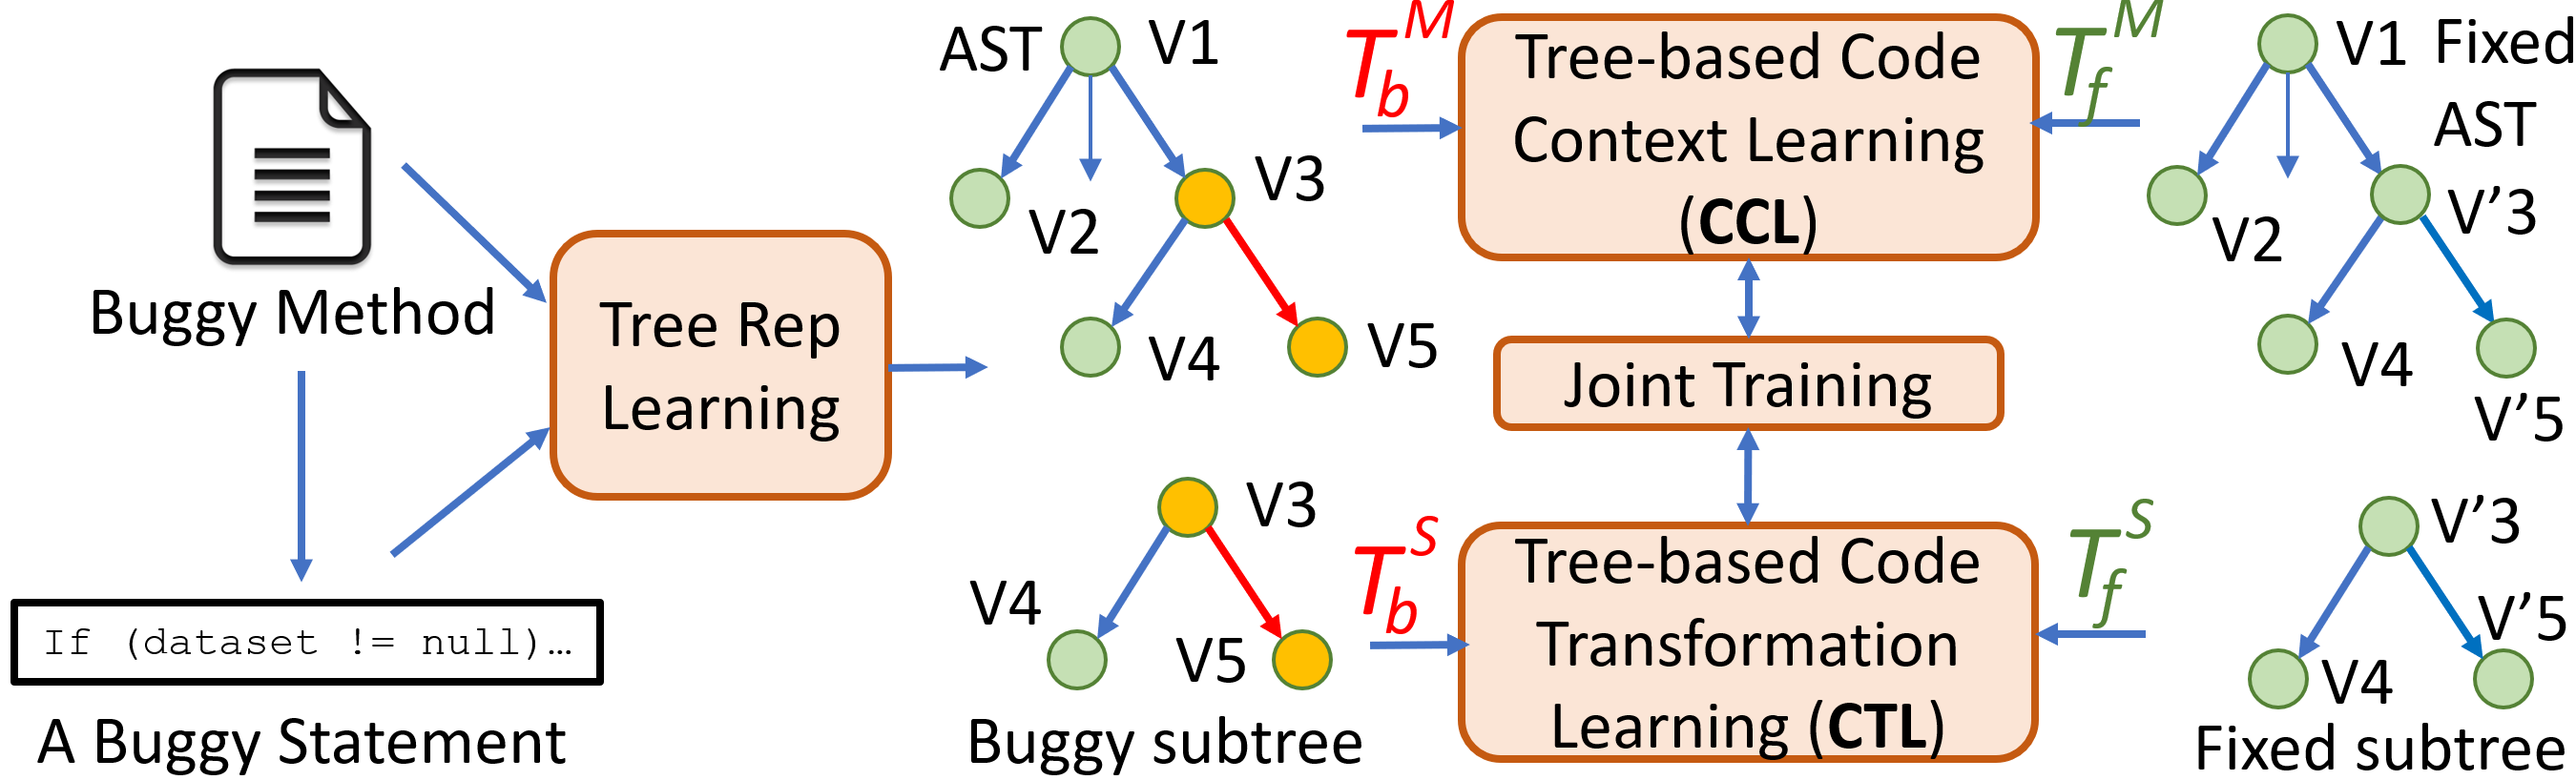
\includegraphics[width=3.4in]{graphs/new_overview-2.png}
        \vspace{-15pt}
	\caption{{\tool}: Training Process}
	\label{overview-training}
%	\vspace{-10pt}
\end{figure}

%\vspace{3pt}
\noindent {\bf Tree-based Representation Learning.} This step aims to
take the source code and to build the tree-based vector
representations (embeddings) to be the inputs of CCL and CTL. To
achieve that, the given method is parsed to obtain its AST
and the subtree for the buggy statement.
%we first parse the given source code to obtain the AST for the given
%method and the subtree for the buggy statement.
Then, the word embedding technique, GloVe~\cite{pennington2014glove},
is used to produce the vector for each node in the AST when we flatten
the AST into a sequence. The output of this step is the AST for the
method and the AST subtree for the buggy statement
in which each node is replaced by its embedding vector
(Figure~\ref{overview-training}).

\vspace{3pt}
\noindent {\bf Context-aware, Dual-Task Learning Automated Program
  Repair.}  The goal of this step is to train both the tree-based CCL
and the tree-based CTL in a joint-training manner. The entire AST
$T^{M}_b$ of the buggy method after vectorization (i.e., each node is
a vector) is used at the input layer of CCL for training. The AST of
the corresponding fixed method $T^{M}_f$ after vectorization is used
at the output layer of the CCL model. Similarly, the AST subtree
$T^{S}_b$ of the buggy statement after vectorization is used at the
input layer of CTL, and the subtree $T^{S}_f$ of the corresponding
fixed statement after vectorization is used at the output layer of
CTL. The CCL and CTL models are realized via attention-based
\code{seq2seq} models.
%Instead of cascading the two models CCL and CTL,
We use the {\em cross-stitch unit}~\cite{misra2016cross} to train CCL
and CTL simultaneously with soft-sharing the parameters to exploit
this duality. Joint training is aimed to learn the shared
representations between CCL amd CTL in terms of a linear combination
of the input features in both models. The output of this step includes
the trained CCL and CTL models.

\subsection{Prediction Process}



Figure~\ref{overview-fixing} illustrates the prediction process, i.e.,
the automated fixing process. A common usage of our tool is that
a developer could first use a fault localization tool
(FL) to detect the buggy statements that need to be fixed. Then, the
input for {\tool} is a buggy statement in the enclosing method.
%Another usage is that a developer can pinpoint the buggy statement and
%invoke {\tool} for an auto-fixing suggestion.
The fixing process shares the first step of Tree-based Representation
Learning with the training process. After that step, the vectorized
buggy AST subtree (each tree node is represented by a vector), is used
as the input of the {\em trained tree-based} CTL. The output of the
trained CTL model is the fixed AST subtree, which is converted back
into source code to form a candidate patch. We design a novel patch
generation that uses beam search over the AST structure and works in
accordance with the decoder as part of CTL in order to improve
efficiency. Finally, we adopt the patch validation process via test
cases as in DLFix~\cite{icse20}.

%the candidate patches are validated and output.

%We design a novel patch validation scheme that makes use of beam
%search for an efficient process. The final candidate patches are then
%produced.

\begin{figure}[t]
	\centering
	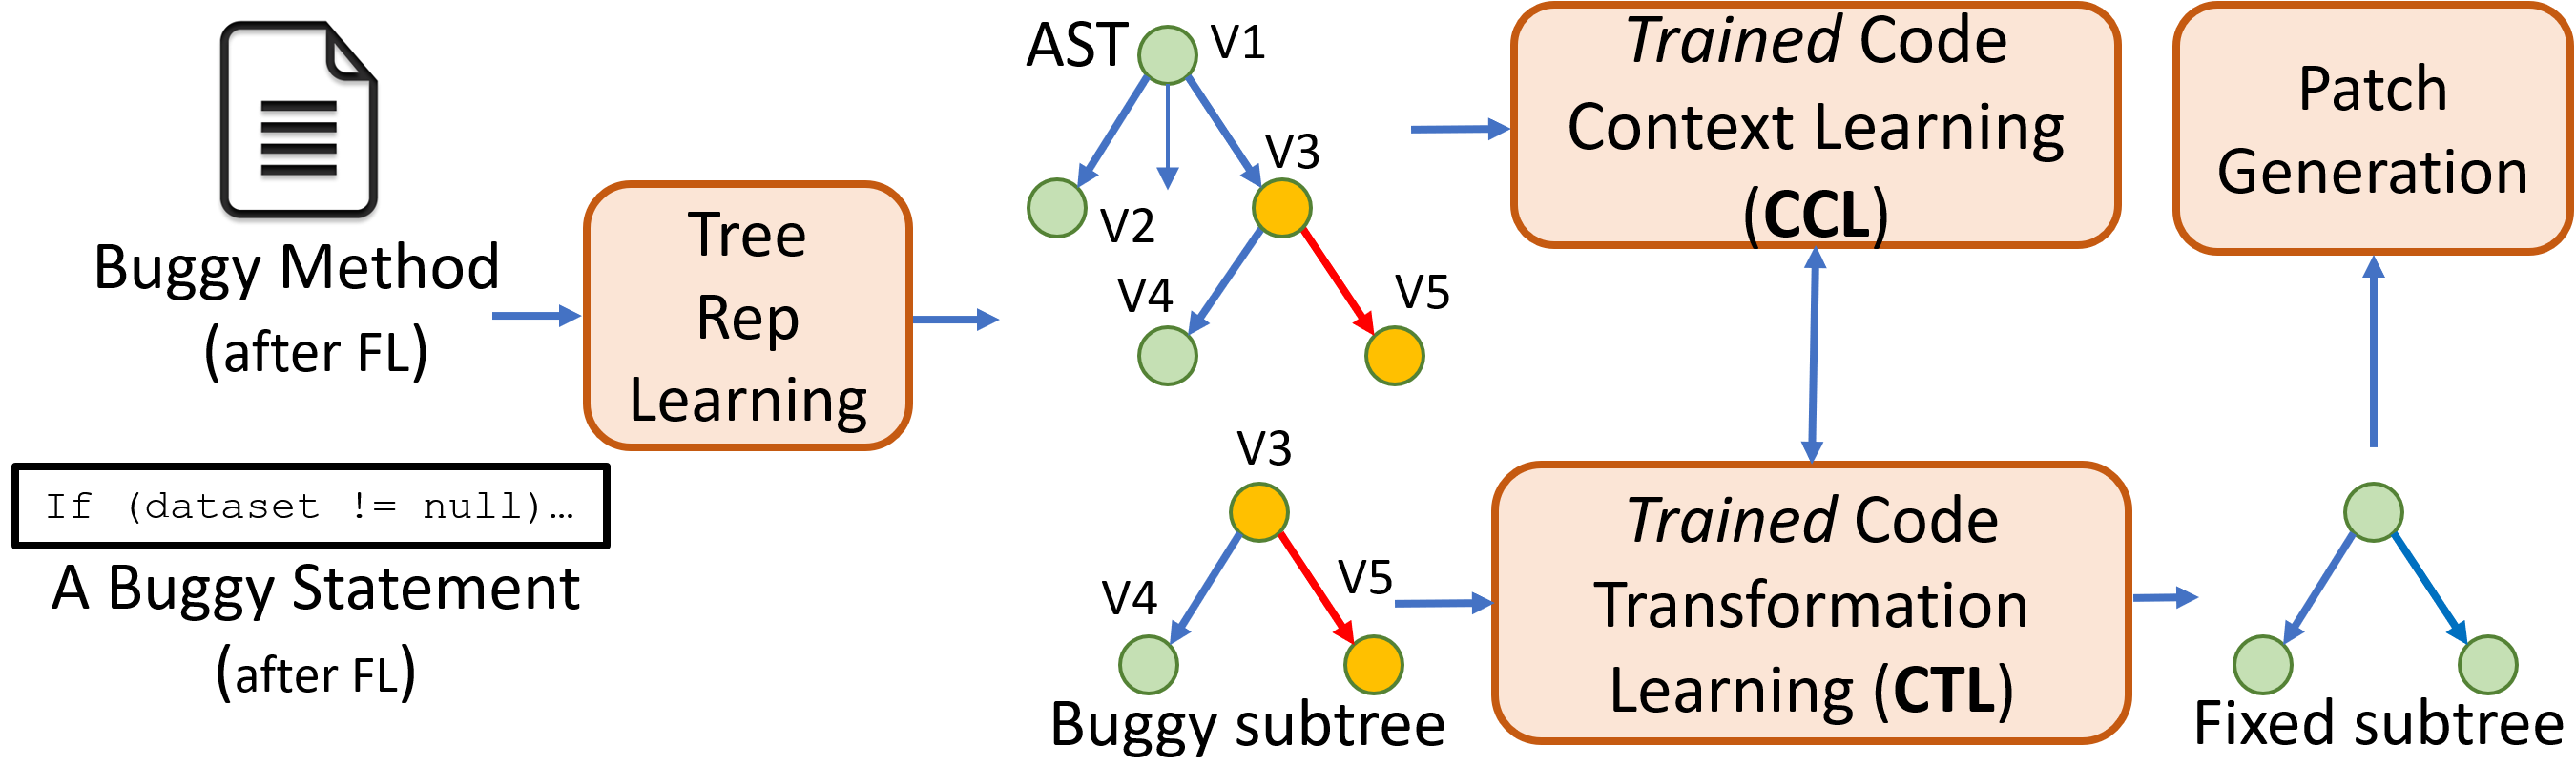
\includegraphics[width=3.4in]{graphs/overview-predict-2.png}
	\caption{{\tool}: Fixing Process}
        \vspace{-3pt}
	\label{overview-fixing}
\end{figure}

\section{Tree-based Representation Learning}

%\begin{figure}[t]
%	\centering
%	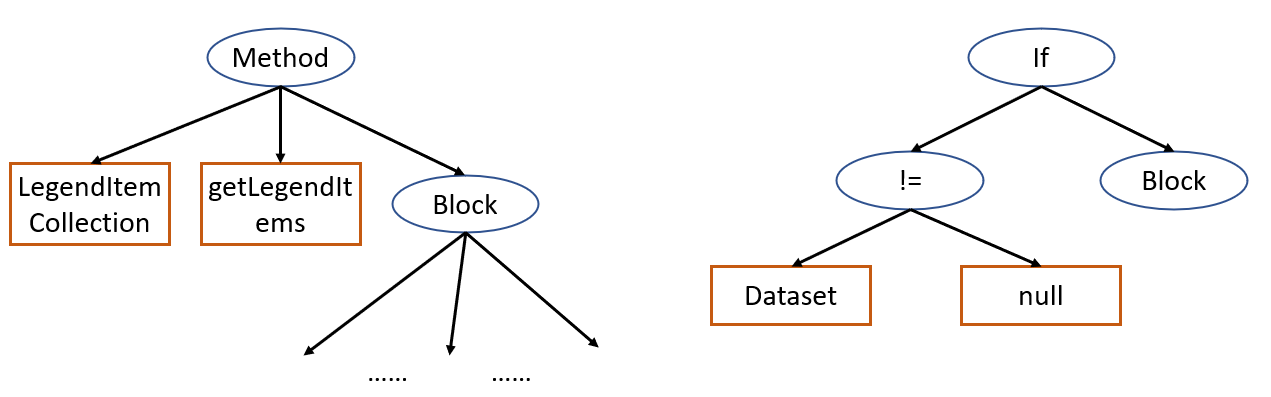
\includegraphics[width=3.2in]{graphs/tree_extraction.png}
%	\caption{Abstract Syntax Tree Extraction Example}
%	\label{tree-extraction}
%\end{figure}

%The goal of this step is to take the source code under study and to
%build the vector representations (embeddings).

This step aims to build the embeddings for the given source code.

\begin{figure}[t]
	\centering
	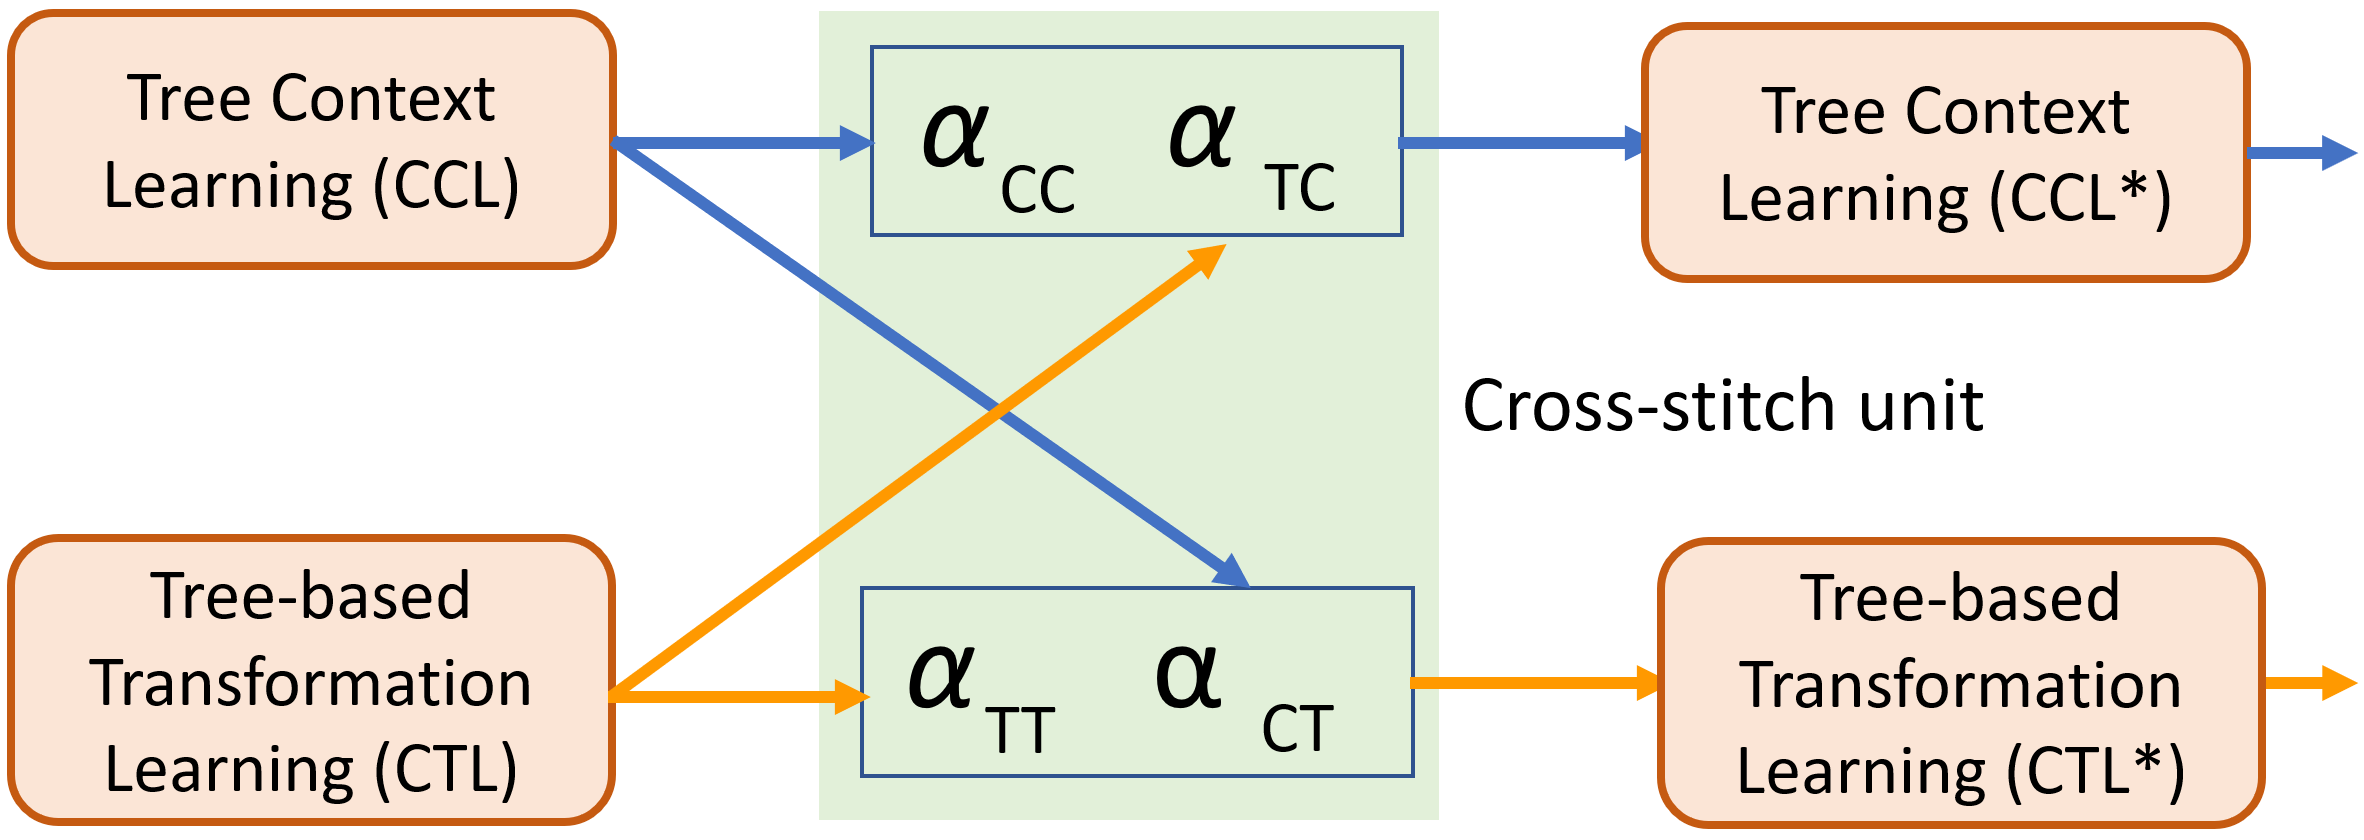
\includegraphics[width=2.8in]{graphs/cross-stitch}
        \vspace{-6pt}
	\caption{Cross-Stitch Unit for Joint Training~\cite{misra2016cross}}
	\label{fig:cross-stitch}
\end{figure}


%\subsection{AST Building and Pairing of Subtrees}

For a buggy method $M$, we parse the code to build the AST for
$M$. We identify the subtree $T_s$ for each buggy
statement $s$. If there are multiple buggy statements~in $M$, we
generate multiple AST subtrees, and use a buggy~statement
together with $M$ as a training instance for CCL and CTL.
%to train the context learning and code transformation models.
We use the tree differencing tool, CPatMiner~\cite{nguyen2019graph} to
identify the respective fixed subtree for the subtree $T_s$ of $s$. We
use them to train CTL. To train CCL, we build the context by
collecting the AST nodes having data and control dependencies with
$s$.

%Second, to train CCL, we take a buggy method $M$ and the corresponding
%fixed version of $M$, and parse them to build the two ASTs.
%However, to train CTL, as shown in Figure~\ref{overview-training}, we
%need to identify the respective fixed subtree for the subtree $T_s$ of
%a buggy statement. To do so, we use the tree differencing tool,
%CPatMiner~\cite{nguyen2019graph}, to derive the fixing changes.

%If a subtree corresponds to a statement, let us call it {\em
%  S-subtree}. From CPatMiner's result, we use the following rules to
%{\em pair a buggy subtree with the corresponding fixed subtree}:

%1. A buggy subtree ($S$-subtree) is a subtree with
%\code{updated}, \code{deleted}, or \code{inserted}.

%2. If a $S$-subtree is \code{deleted}, we pair it with an empty tree.

%3. If a buggy $S$-subtree is marked as \code{updated}, (i.e, it is
%{\em updated} or its children node(s) could be {\em inserted, deleted} or {\em
%  updated}), we paired this buggy $S$-subtree with its corresponding
%fixed $S$-subtree.

%4. If a $S$-subtree is \code{inserted} and its parent node is another
%$S$-subtree, we pair it with that parent $S$-subtree.  If the parent
%node is not an $S$-subtree, we pair an empty tree to the corresponding
%inserted $S$-subtree.
%------------------------------------------------



%The first step of the \tool is the tree extraction step designed to extract abstract syntax tree (AST) from the source code. It accepts the buggy method with the changed statements inside as input. The output of this step is the extracted AST for the whole buggy method and the extracted subtree of AST that represents the changed statements.

%Specifically, for a buggy method $m$, \tool uses the Java package JDT \cite{JDT} to generate the AST $Tree_m$ to represent the buggy method. And for a buggy statement $s$ in the buggy method, \tool uses the subtree of AST $Tree_s$ that exactly covers the statement $s$ to represent the buggy statement. For example, in Figure \ref{tree-extraction}, the AST in the left represents the buggy method in Figure \ref{fig:motiv}, and the right subtree of AST in Figure \ref{tree-extraction} represents the buggy statement. If there is more than one buggy statement in the buggy method $m$, \tool generates multiple subtree of AST to represent each buggy statement.

%Also, when training the model, \tool needs ground truth to let the model learn the parameters, \tool also generates the AST $Tree_{mf}$ to represent the fixed method $m_f$ and the subtree of AST $Tree_{sf}$ to represent the fixed statement $s_f$. Here, $m_f$ is the after fixing version of buggy method $m$, and $s_f$ is the after fixing version of buggy statement $s$. Thus, \tool uses the AST and subtree of AST for fixed method and fixed statement as the ground truth to train the model parameters.

%For the buggy method, $m$ and corresponding fixed method $m_f$, \tool can easily find them from the dataset based on the true labels. However, pairing the buggy statement $s$ with its corresponding fixed version $s_f$ is not easy as the methods. To solve this problem, we use an existing approach CPatMiner \cite{nguyen2019graph} to process the fixing changes. Based on the results from CPatMiner, we pair the buggy statement $s$ with the corresponding fixed statement $s_f$ within the three following conditions. 1) If the buggy statement $s$ needs to be deleted, we pair $s$ with an empty statement. 2) if the buggy statement $s$ needs to be updated, we pair $s$ with the updated statement. 3) If there needs to insert a new statement as the fixing, we check the AST for the method $m$ first. And we pair the parent node with the inserted statement $s_f$ if the parent node representing the other statement, or we pair an empty statement with the inserted statement $s_f$.

%\subsection{AST Node Representation Learning}

To provide the compatible inputs for CCL and CTL models, we need to
perform an AST node representation learning process in which each node
in the AST subtree or the AST of the method is replaced by the
embedding of the node. To achieve that, we first flatten the AST
subtree under study by a depth-first-search traversal to obtain a
sequence of tokens. For the case of an AST subtree, we consider the
sequence of tokens of a $S$-subtree as a sentence. For the case of the
AST of the method, we consider the sequence of tokens for the method
as a sentence. We then use a word embedding technique
%GloVe~\cite{pennington2014glove}
to run on those sentences to build a vector representation for each
token, i.e., for each AST node in the method's AST or in the AST
subtree. (Our implementation uses GloVe~\cite{pennington2014glove}).
%We used GloVe because it can capture well the co-occurrences
%among tokens~\cite{pennington2014glove}. After running GloVe,
We then replace each node in the (sub)tree with its vector
representation (Figures~\ref{overview-training}
and~\ref{overview-fixing}). Similarly, we replace each node with its
vector in the AST of the fixed method and in the AST subtree of the
fixed~statement.

%To make the dual learning program repair model can take information from the input, \tool firstly needs to vectorize the AST and the subtree of AST by using the node representation learning.

%For a given tree $T$, \tool firstly uses the deep traversal to covert it into a sequence of tokens $S$. Here, $T$ could be $Tree_m$, $Tree_{mf}$, $Tree_s$, and $Tree_{sf}$. And then, \tool uses the famous technique GloVe \cite{pennington2014glove} to transform each AST node into a vector. The GloVe is a great tool for vectorizing the sequence of tokens by considering co-occurrence between different tokens. It can help predict for the often appeared together tokens. That's the reason why to choose it here to vectorize the tree $T$. For example, in Figure \ref{program-repair}, the AST node $N1-N5$ has been embedded into the vector $V1-V5$ in the top raw.

\section{Dual Learning Program Repair}

\begin{figure}[t]
	\centering
	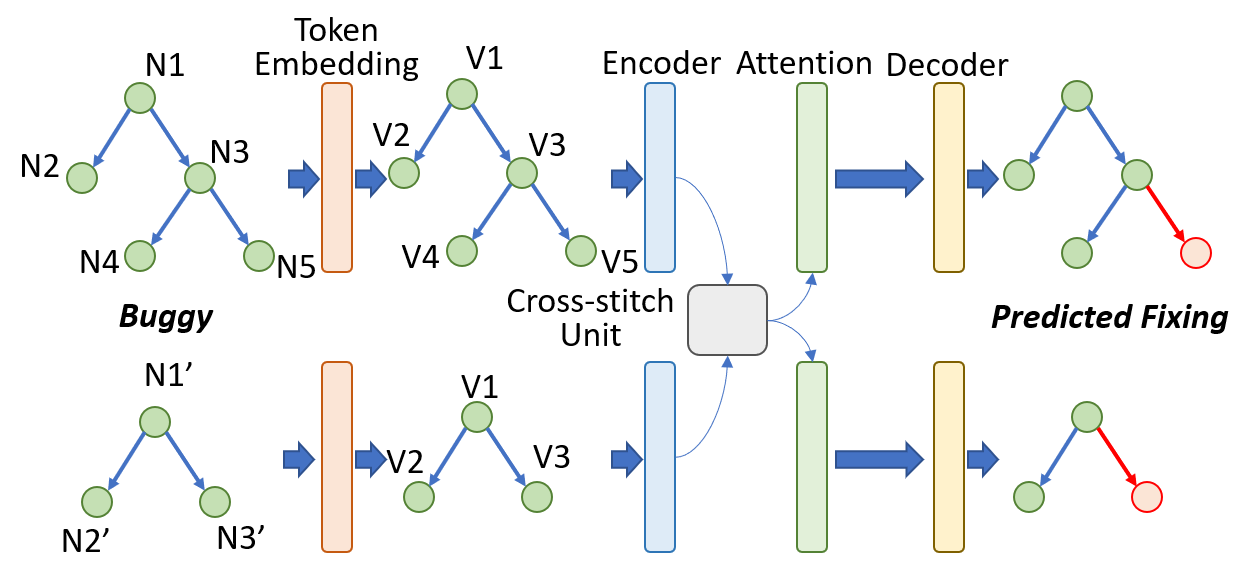
\includegraphics[width=3.2in]{graphs/program_repair.png}
	\caption{Dual Learning Program Repair}
	\label{program-repair}
\end{figure}

After having the $Tree_m$, $Tree_{mf}$ pair and $Tree_s$, $Tree_{sf}$ pair from the first step, \tool uses them as the input and the ground truth to train the dual learning program repair model in this step. \tool uses the generated after fixing AST $Tree'_m$ and after fixing subtree of AST $Tree'_s$ as output for this step when making the prediction. Specifically, there are two small steps, including the AST node representation learning and the dual learning framework.




\subsection{Dual Learning Framework}

First, \tool uses two separate attention-based seq2seq frameworks to learn the code fixing for both the method-level and the statement-level. We all use the tree-based deep learning model to process the AST or subtree of AST for the encoder and decoder of these two tasks. Based on the recent study, we select a well-performed baseline TreeCaps \cite{bui2021treecaps} here to do so. Between the encoder and decoder, there is an attention layer for both tasks to help improve the accuracy of generating the fixing.

In the regular attention-based seq2seq model, the hidden status $H$ is directly passed to the attention layer. However, \tool uses a cross-stitch unit to accept the hidden status $H_m$ and $H_s$ from both method-level and the statement-level to achieve the dual learning. And then, the \tool passes the output of the cross-stitch unit to the method-level and statement-level attention layer. Just like the Figure \ref{program-repair} shown, the output from the encoder does not go to the attention layer. They go to the cross-stitch unit instead. The cross-stitch unit helps both the method-level and the statement-level attention-based seq2seq model catch the input features within the buggy method and the buggy statement.

As for the TreeCaps model \tool is using, it is built on top of $k$ TBCNN layers \cite{mou2014tbcnn}. So, for the TBCNN layer $k$, the output of the convolution window is calculated as:

\begin{equation}\label{eq:1}
	Y = tanh(\sum_{i=1}^{N}[\Delta^t_iW^t + \Delta^t_iW^t + \Delta^t_iW^t]X_i + b)
\end{equation}

Where $\Delta$ are weights calculated corresponding to the depth and the position of the nodes. One can see this as a
way to learn the position of a node inside AST. $W$ is the trainable matrix; $b$ is the bias; $N$ is the total number of nodes in the convolution window. TreeCaps merges the output from all TBCNN layers by using a non-linear squash
function \cite{sabour2017dynamic}. For an AST node $j$, we calculate the capsules $u_j$ as:

\begin{equation}\label{eq:2}
	u_j = \frac{||c_j||^2}{||c_j||^2+1}\frac{c_j}{||c_j||}
\end{equation}

By merging all capsules as a list with the deep traversal order, \tool has the output $H$ for the TreeCaps model.

After \tool has $H_m$ and $H_s$ for both method-level and statement-level in the encoder, we aim to learn the linear combinations of both inputs of the cross-stitch unit. The output of the cross-stitch unit is computed as:

\begin{equation}\label{eq:3}
	\begin{bmatrix}
		X_m\\
		X_s
	\end{bmatrix}
	=
	\begin{bmatrix}
		\alpha_{mm} &  \alpha_{ms} \\
		\alpha_{sm} &  \alpha_{ss}
	\end{bmatrix}
	\begin{bmatrix}
		H_s\\
		H_m
	\end{bmatrix}
\end{equation}

Where $\aleph$ is the trainable weight matrix, $X_m$ and $X_s$ are the inputs for the attention layers of both two tasks. For $X_m$ and $X_s$, they both contain the information learned from the method-level and the statement-level, which achieves the main goal of the dual learning framework. From formula \ref{eq:3}, we could know:

\begin{equation}\label{eq:4}
	X_m = \alpha_{mm}H_m + \alpha_{ms}H_s
\end{equation}
\begin{equation}\label{eq:5}
	X_s = \alpha_{sm}H_m + \alpha_{ss}H_s
\end{equation}

However, if the $H_s$ and $H_m$ have different sizes, we need to resize them to be consistent. If the size needs to be increased, we use the bilinear interpolation for resizing. If the size needs to be reduced, we do the center crop on the matrix to match the required size.

After solving this, here is one last problem the dual learning may face. When making the prediction, because we don't know how the tree structure changes, \tool needs to have a size limit to control the fixing. \tool expands the child node number to $P$ and expands the child node depth to $Q$ for a buggy node. It means that we make each buggy node have at most $P+P^2+...+P^Q$ nodes. When making predictions, if one node is close to zero, we think it is empty and drop it. At the same time, all child nodes of it will be dropped by \tool.

\section{Patch Generation}
\label{sec:patch-gen}

Figure~\ref{overview-fixing} shows the overview of the fixing process.
While the steps of parsing and tree-based representation learning are
the same as in the training process, the step of applying the trained
\code{CCL} and \code{CTL} models to produce the candidate patches is
different. Let us detail that step, which is illustrated in
Figure~\ref{fig:patch-gen}.

As explained earlier, the output of the cross-stitch unit connects to
the attention layer, which in turn connects to the decoder. The
decoder has four main components: 1) the embedding component to encode
the input at a time step into the subtree whose nodes are vectors; 2)
the TreeCaps~\cite{bui2021treecaps} component to summarize the vectors
in a subtree into a vector; 3) the output layer; and 4) the beam
search component, which takes the output at the output layer and
produces a candidate patch in terms of the output AST subtree $T_i$
with the concrete source code for the nodes at the current time step
$i$.  While the embedding component, TreeCaps, and the output layer
are straightforward, we need to explain the adaptation we have made in
the beam search component.

Beam search is an optimization strategy to keep only the top-$K$ best
solution for the output subtree $T_i$ at a time step $i$ to help
reduce the search space. The reason that we need to use a beam search
strategy is that at each node when we convert a vector back to a code
token, we might have multiple candidate tokens for each node. For
example, in Figure~\ref{fig:patch-gen}, we might have multiple
candidate code tokens for the nodes $N_1$, $N_2$, and $N_3$. Thus, we
might face the combinatorial explosion when considering all the nodes
in the output subtree $T_i$ at each time step $i$.

Because the beam search component aims to produce the subtree to be
used as the input of the decoder at the next time step $i+1$
(Figure~\ref{fig:patch-gen}, it must work in accordance with the
TreeCaps component. TreeCapscomputes the vector from bottom up (i.e.,
the vectors for children nodes are computed before the one for their
parent node). Therefore, our beam search component considers the order
of the nodes in the AST subtree from the bottom up first, and for the
left-to-right order of the sibling nodes of the same parent node. For
example, for the tree $V1$--$V5$ in Figure~\ref{overview-training},
the beam search component will consider the order of the nodes as
follows: $V2$, $V4$, $V5$, $V3$, and $V1$. The sequences of code
tokens in that order for the AST nodes are considered. The score for a
sequence is the product of the probabilities of all the nodes. At each
step, the sequences are ranked and only the top-$K$ best sequences are
maintained.

Another issue occurs during the conversion from an embedding to a code
token. When we search in our dictionary for a token that has a vector
closest to the vector of the current node under consideration, we
might encounter a token that is not in the same project or invalid for
the current scope of the program. Thus, we perform static analysis
with several filters to keep only the valid tokens in the current
scope. Specifically, we apply a set of filters to verify the program
semantics as in DLFix~\cite{icse20}. We use the alpha-renaming filter
to change the names back to the normal Java code using a dictionary
containing all the valid names in the scope, the syntax-checking
filter to remove the candidates with syntax errors, and the name
validation filter to check the validity of the variables, methods, and
classes.

Afterward, \tool runs the corresponding test cases for the bug
$b_i$. If there is any test case failed, \tool attempts the next
candidate. If all test cases pass, we regards the candidate as
a correct fix.

%The first problem is that when transferring the predicted fixing to
%the real tokens, beam search uses the GloVe embedding
%dictionary. However, this dictionary is learned from multiple
%projects. So the invalid tokens may be generated by the beam
%search. So \tool creates a rule that before using the beam search,
%\tool firstly makes static analysis to select all appeared token in
%the project and when doing the beam search, the results only come from
%the appeared token set.

%Secondly, because the beam search is designed for sequential data,
%\tool makes some small changes to work on the tree structure. To be
%more detailed, \tool regards the nodes with the same parent node as
%the same level. And when doing the beam search, \tool considers these
%nodes at one time by multiply the possibility score for each node. The
%beam search order is from the bottom to the top, which means the node
%with a higher height will be considered first.

%For example, in Figure \ref{patch-validation}, the AST node $N3$ and
%$N4$ will be considered the first when doing beam search. If the
%possibility of $N3=Dataset$ is $p_1$ and the possibility of $N4=null$
%is $p_2$. The first step of beam search will have an optimal token
%like $N3=Dataset, N4=null$ with the possibility of $p_1*p_2$. The
%second step of the beam search is to search $N2$ and $N5$ in the dark
%box simultaneously. And the last step of the beam search is dealing
%with the node $N1$ in the orange box.


%This step will only be used during the prediction, and because the statement-level program repair is our main goal for the dual learning, \tool only consider the output from the statement-level here. After \tool has the predicted fixing for the subtree of AST $Tree_s$, \tool uses the beam search to help the model reduce the search space and run the test cases to do the validation. Beam search is an optimized greedy strategy, and Beam search keeps only the $n$ optimal tokens for each step to help reduce the search space. However, there are two problems the beam search may face when applying to \tool to do the validation.





%After doing the beam search, \tool runs the corresponding test cases for the bug $b_i$. If there is any test case failed, \tool tries the second candidate for the fixing. If all test cases passed, \tool regards the current candidate as the correct fixing for the bug $b_i$, which is the final output for the \tool.

\begin{figure}[t]
	\centering
	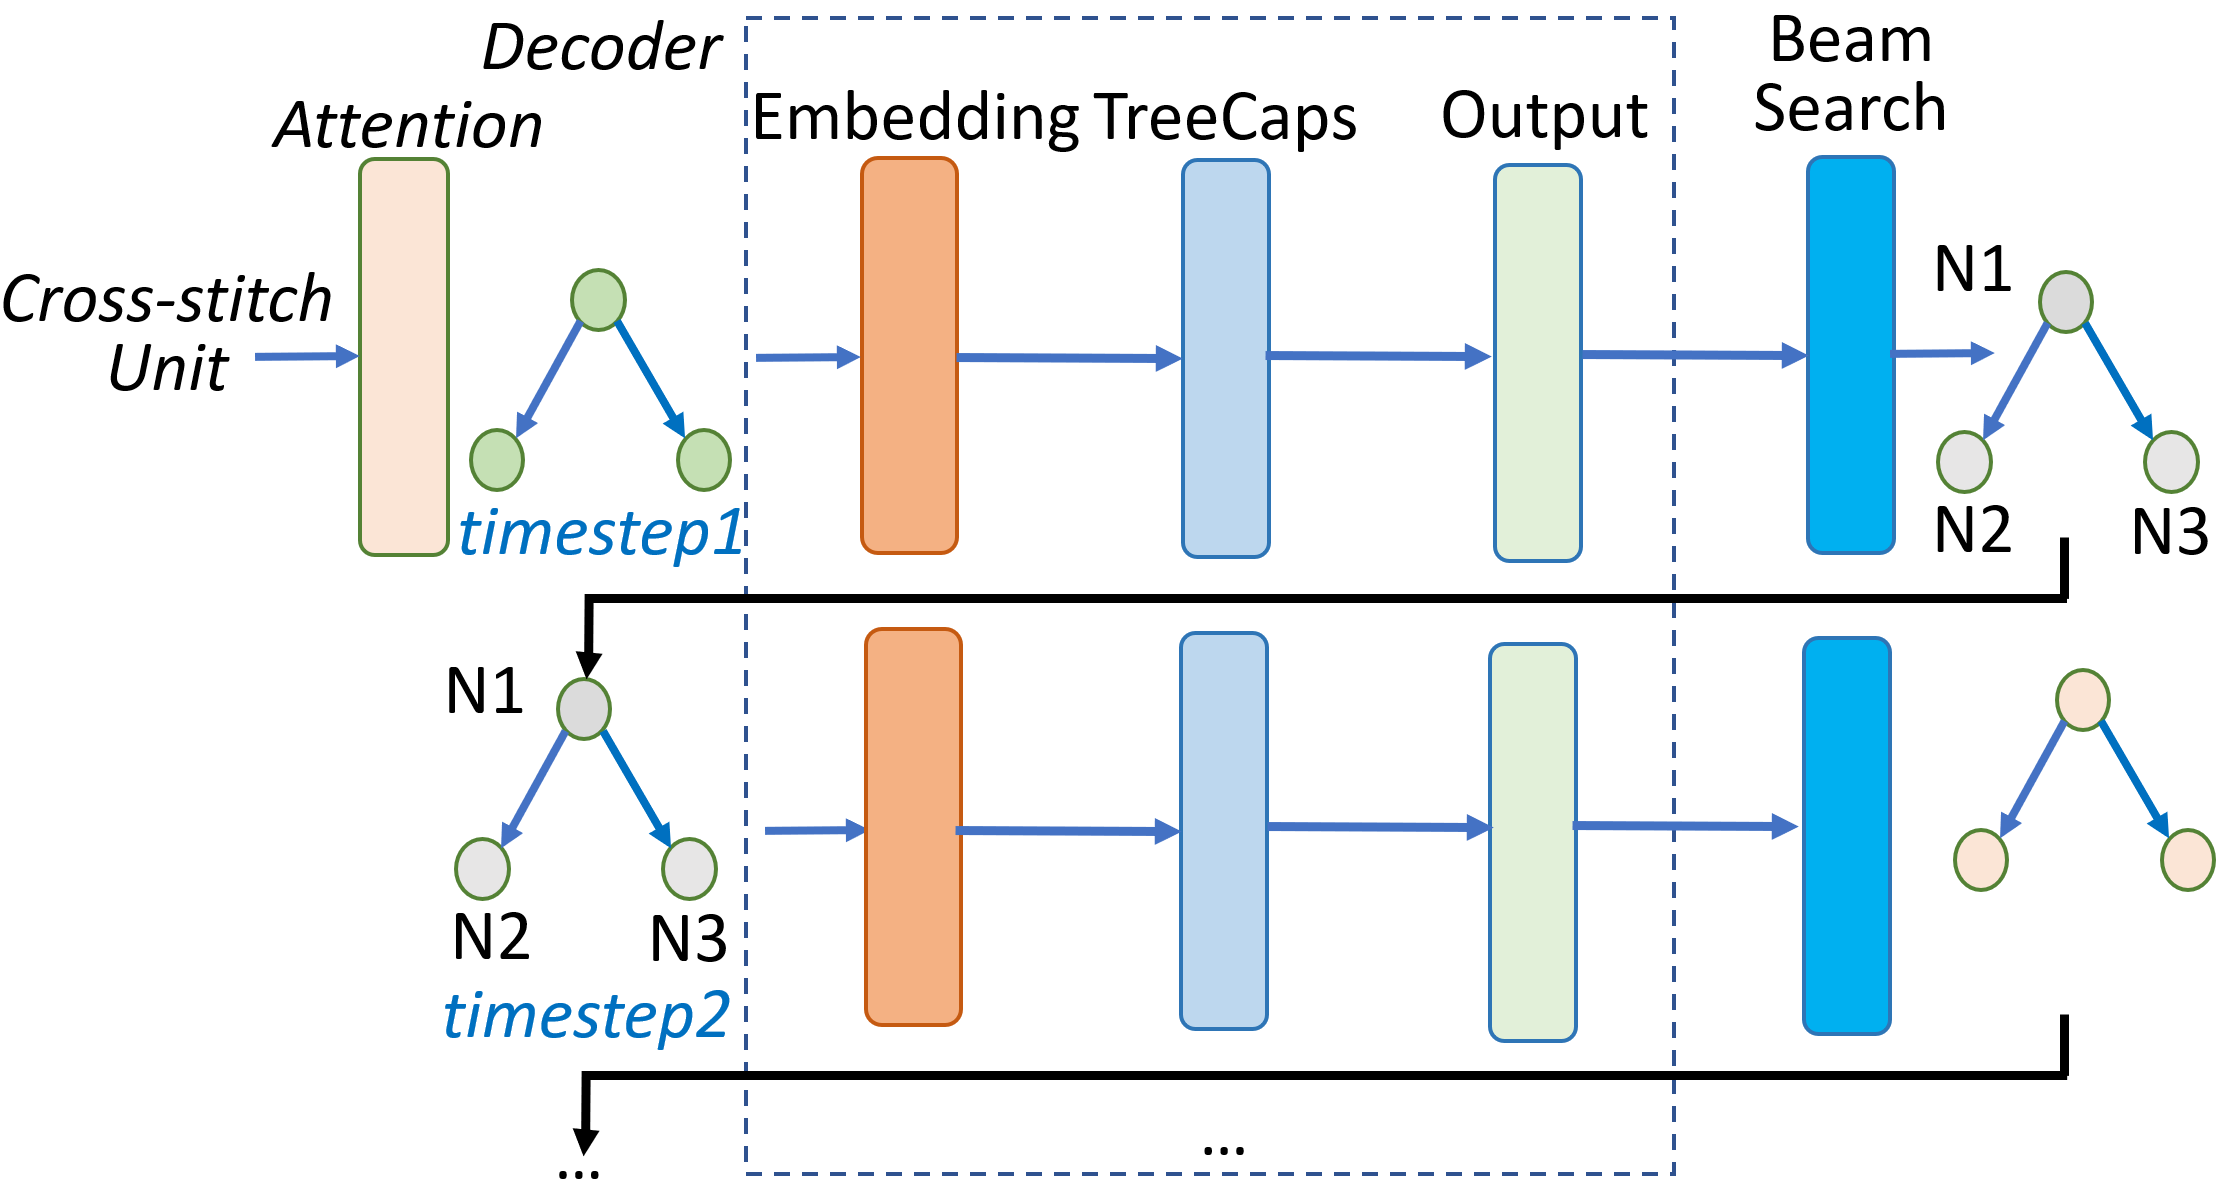
\includegraphics[width=3.2in]{graphs/beam-search.png}
	\caption{Patch Generation via Tree-Structured Beam Search}
	\label{fig:patch-gen}
\end{figure}

\section{Empirical Evaluation}

\subsection{Research Questions}

We seek to answer the following research questions:

\noindent\textbf{RQ1. Comparison with State-of-the-art APR Approaches on Defects4J Dataset.}  How well does {\tool} perform compared with the state-of-the-art automate program repair approaches on Defects4J dataset?


\noindent\textbf{RQ2. Comparison with State-of-the-art APR Approaches
  on Large Datasets.}  How does {\tool} perform compared with the
state-of-the-art automate program repair approaches on large datasets?


\noindent\textbf{RQ3. Overlapping Analysis.} How many bugs that
{\tool} can fix that the other DL-based baselines
                missed and vice versa?

\noindent\textbf{RQ4. Impact Analysis of Dual-learning Model.} How does the dual learning model affect the overall performance of {\tool}?


\noindent\textbf{RQ5. Evaluation on C Projects.} How does {\tool} perform on C projects?

\subsection{Empirical Methodology}

\subsubsection{Datasets}
We perform our valuation on three datasets that have been used
in the prior research in APR~\cite{icse20}:
Defects4J~\cite{defects4j}, Bugs.jar~\cite{saha2018bugs}, and
BigFix~\cite{yioopsla19}. The version of the Defects4J dataset we used
in this study is the V1.2.0~\cite{defects4j} with 395 bugs
from 6 Java projects. For each bug in a project, Defects4J has the
faulty and fixed versions of the project. There are relevant test
cases for each bug. With the \code{Diff} comparison between faulty and
fixed versions of a project, we can identify the buggy statements. The
Bugs.jar dataset contains 1,158 bugs and patches from 8 large, popular
open-source Java projects. The BigFix dataset contains +4.9 million
Java methods, and among them, +1.8 million Java methods are
buggy. There are also the corresponding bug fixes for the buggy
methods in each dataset as in Defects4J. We conducted all the
experiments on a server with 16 core CPU and a single Nvidia A100 GPU.

\subsubsection{Evaluation Metrics}

We use three evaluation metrics to evaluate the performance of \tool
and the baseline models.

{\bf 1. Correct Patches/Plausible Patches:} Correct patches are the
fixes that exactly match or have the same semantic meaning as the
fixes in the ground truth by real developers. Plausible patches are
the fixes that pass all the test cases, but might not match exactly
with the actual fixes by developers.

%It may contain the correct patches and the situation that
%the generated fixing is not correct but passes all test cases.
{\bf 2. P\%:} is the percentage of generated plausible patches to
be correct ones matching the ground truth by real developers.

{\bf 3. Top-$K$:} is the percentage of total bugs in which a correct
patch for a bug is in the ranked list of top-$K$ candidate patches.

\subsubsection{Evaluation Methodology.}
We use the following settings for different RQs:

{\bf RQ1. Comparison with the state-of-the-art DL-based APR Approaches on
  Defects4J Dataset.}

\underline{Baselines.} We compare {\tool} with the following
state-of-the-art deep learning (DL)-based APR baseline models:

%{\it Hercules \cite{hercules-icse19}: } is a novel APR technique that generalizes single-hunk repair to encompass a specific but significant class of multi-hunk repair problems.

%{\it Tbar \cite{tbar-issta19}: } is a template-based APR to build comprehensive% knowledge about the effectiveness of fix patterns.

{\bf SequenceR~\cite{chen2018sequencer}: } uses the machine
translation approach with sequence-to-sequence learning.

{\bf CoCoNuT~\cite{lutellier2020coconut}:} uses a context-aware neural
machine translation architecture to represent the buggy source code
and its surrounding context separately. However, it does not have the
dual learning for context learning and code transformation learning as
in {\tool}. It uses ensemble learning on the combination of
convolutional neural networks and a context-aware machine translation.

{\bf DLFix~\cite{icse20}: } is a two-tier DL-based model that
treats APR as code transformation learning from the prior bug fixes
and the surrounding code contexts. It follows a cascading architecture
between two models of context learning and transformation learning.

{\bf CURE~\cite{cure-icse21}: } is a machine-translation-based program repair
technique that by design parses, models, and searches source code, as
opposed to natural language text, to fix bugs automatically. It treats
context separately from the buggy statements as in CoCoNuT. It does
not have the dual learning for context learning and code
transformation learning as in {\tool}.


%Tien
%In this RQ, for %Hercules and
%Tbar, we directly use the results reported in their original paper because they are pattern-based approaches.

For all approaches under study in this RQ, we used the BigFix as the
training dataset and evaluated on Defects4J dataset. 
%For each bug in Defects4J, we used the remaining bugs in Defects4J as the developing dataset to fine-tune the model, and used the fine-tuned model to predict the fix for the bug. 
We used the correct fixing locations for the models to perform fixing
and used test cases for validation steps.  We set a 5-hour limit for
the validation step for all approaches as in previous
work~\cite{icse20,tbar-issta19}.


\underline{Parameter tuning.} We tuned the baselines with the
parameters that mentioned in their papers. We tuned \tool with the
following parameters: {\em epoch}, {\em batch size}, {\em learning
  rate}, {\em embedding length}, the {\em max number of children nodes
  $P$}, {\em the max children node depth} $Q$, and {\em the beam
  search size $n$}. Our model was tuned with the following key
hyper-parameters to obtain the best performance: (1) Epoch size (i.e.,
100, 200, 300); (2) Batch size (i.e., 64, 128, 256); (3) Learning rate
(i.e., 0.001, 0.003, 0.005, 0.010); (4) Vector length of word
representation and its output (i.e., 150, 200, 250, 300).

{\bf RQ2. Comparison with State-of-the-art DL-based APR Approaches on
  Large Datasets.}

\underline{Baselines.} We compare {\tool} with the following state-of-the-art DL-based APR baseline models:

{\bf SequenceR~\cite{chen2018sequencer}, CoCoNuT~\cite{lutellier2020coconut}, DLFix~\cite{icse20}, CURE~\cite{cure-icse21}:} as explained in RQ1.

{\bf CODIT~\cite{chakrabortycodit}:} is the DL-based APR approach using
sequence-to-sequence machine translation model with the abstractions on tree
structures to learn the code transformations for bug fixing.

{\bf Tufano'19~\cite{tufano2019learning}:} is also a DL-based approach
aiming to learn code changes by adopting neural machine translation
with code abstractions and filtering via program analysis.

We did not compare with CODIT~\cite{chakrabortycodit} and
Tufano'19~\cite{tufano2019learning} in RQ1 on Defects4J dataset,
because they do not have the validation step in their approaches to
run on Defects4J. It is unfair if we compared them with the other
approaches having the validation step.

We compared {\tool} with those two baselines in this experiment for
RQ2 running on two large datasets, in which we directly ran the fixing
step without the validation. The two large datasets do not contain the
corresponding test cases for the bugs. Thus, we ran a model
without the validation step on these two datasets.

%The two new baselines in this RQ, including Tufano 19\' and CODIT are not designed for the Defects4J dataset, and there is not validation step in these two approaches. Therefore, comparing these two approaches to other baselines and \tool with the validation step is not fair. So we did not compare these two approaches as baselines in RQ1.

%As for this RQ, for all baselines and \tool, we directly run the
%fixing step without validation. So it is fair to add these two
%baselines.

%We ran the baselines and \tool on two big datasets in this RQ, including Bugs.jar and BigFix.

In this RQ2, as running a model on each dataset, we randomly splitted
it into 80\%/10\%/10\% for training, developing, and testing. We used
the same slitting scheme for all models.


\underline{Parameter tuning.} We tuned the baselines with the
parameters mentioned in their papers and tuned {\tool} in the same
manner as in RQ1 with autoML \cite{NNI}.

{\bf RQ3. Overlapping Analysis.} To further study the comparative
result between a baseline model $M$ and {\tool}, we analyzed and
counted the number of bugs that were fixed by {\tool} and were missed
by $M$, the number of bugs that were fixed by $M$ and were missed
by {\tool}, and the number of bugs that were fixed by both.


{\bf RQ4. Impact Analysis of Dual-learning Model.}

\underline{Baselines.} To study the contributions of dual-learning in
{\tool}, we built two variants:

(1) \textbf{Transformation-only model:} In this variant, the
context learning model is removed from {\tool} and only the bug-fixing
code transformation learning model is kept. The result allows us to
understand the contributions of the context learning model (CCL).

%for training in step 2 of \tool.

(2) \textbf{Cascading model:} We also built another variant model in
which we removed the cross-stitch unit for dual learning, and we
connected the context learning model (CCL) to the transformation
learning model (CTL) in a cascading manner as in DLFix~\cite{icse20}
(the context learning result is added as an additional input of the
transformation learning model).

%the other naive model, the
%two-tier model, as the baseline. As for the two-tier model, we removed
%the dual-learning from {\tool} and make the statement-level program
%repair is dependent on the output of the method-level program repair.

In this RQ, we used the same process and parameter tuning as in the
experiments for the other RQs. We run all models on BigFix.

%the baselines and \tool in this RQ. Therefore, the parameters that
%eed to be tuned in both baselines are the same as the ones of \tool.

{\bf RQ5. Evaluation on C/C++ Projects.}  To evaluate {\tool} on C/C++
code, we ran it on the C/C++ benchmark
Codeflaws~\cite{tan2017codeflaws} with 3902 bugs. 
We used the same process and setting as in RQ2.

\section{Experimental Results}

\subsection{\bf RQ1. Comparison Results with DL-based APR Approaches on Defects4J Dataset}

Table~\ref{RQ1_defect4j} shows that {\em {\tool} can auto-fix more bugs
than any DL-based baselines}. {\tool}
automatically fixes 56 bugs and it fixes {\bf 194.7\% (i.e., 37), 40\%
(i.e., 16), 27.3\% (i.e., 12), and 16.7\% (i.e., 8)} more bugs than the
baseline models SequenceR, DLFix, CoCoNuT, and CURE,
respectively.
%{\color{red}{if add CURE*, this is not true}}
Furthermore, {\tool} generates {\em the most plausible
patches (i.e., 96)} passing all test cases than any other baselines,
indicating that {\tool} has a better patch generation
capability. Moreover, {\tool} has a {\em higher percentage of the generated
plausible patches to be correct than all the baselines}, except
SequenceR. However, {\tool} can fix 194\% more bugs and 6 times more
plausible patches than SequenceR.
%
 %and CURE fixed 4 bugs that {\tool} missed. 
% {\tool} fixed 12 unique bugs that CURE cannot fix and 3 unique bugs
% that were missed by all other baselines.
Moreover, CDFix fixed 12 bugs that the {\em best baseline} CURE
missed; and CURE fixed 4 bugs that CDFix missed. CDFix fixed 3 bugs
that all the DL-based baselines missed.

Table~\ref{RQ1_defects4J_with_FL} shows the comparative result on
Defects4J with an FL tool. As seen, with the FL tool, the performance
of all models decreases due to the confounding inaccuracy. However,
{\tool} can still fix more bugs than any baseline. It
automatically fixes {\bf 44} bugs, i.e., {\bf 193.3\% (i.e., 29), 46.7\%
  (i.e., 14), 33.3\% (i.e., 11), and 22.2\% (i.e., 8)} more bugs than
the baselines SequenceR, DLFix, CoCoNuT, and CURE,
respectively.
%{\color{red}{if add CURE*, this is not true}}
Furthermore, {\tool} generates the most plausible patches (i.e., {\bf
  XX}) among all the models.
%indicating that {\tool} has a better patch generation
%capability. Moreover, {\tool}
It also has a higher percentage of the generated plausible patches to
be correct than all the baselines.
%However, {\tool} can fix 194\% more bugs and 6 times more plausible
%patches than SequenceR.
Moreover, CDFix fixed {\bf 9} bugs that the {\em best baseline} CURE
missed; and CURE fixed {\bf 3} bugs that CDFix missed. CDFix fixed
{\bf 2} bugs that all the DL-based baselines missed.

Note that the numbers for DLFix are different from those
reported in DLFix paper~\cite{icse20}. The reason is that DLFix's
authors had filtered from the datasets the multiple-line bugs due to
DLFix's limited capabability. We used the full datasets with all the
bugs.

%Tien
%The reason for the difference between the results for DLFix in this paper and those reported in DLFix’s paper_[18] is that in DLFix’s experiment, the authors filtered from the datasets to keep only the single-line bugs for the comparison with other baselines. In CDFix, we used the full datasets with multiple-line bugs. Thus, the results reported in this paper are lower. The same reason is for other baselines.



%{\footnotesize{
\begin{table}[t]
  \caption{RQ1. Comparison Results with DL-based APR Approaches on Defects4J \underline {without Fault Localization}.}
  \vspace{-6pt}
  {\small
			\begin{center}
				\renewcommand{\arraystretch}{1}
				\begin{tabular}{p{0.8cm}<{\centering}|p{1.2cm}<{\centering}|p{0.9cm}<{\centering}|p{1cm}<{\centering}|p{0.8cm}<{\centering}|p{0.8cm}<{\centering}|p{0.8cm}<{\centering}}
					
					\hline
					&\textbf{SequenceR}&\textbf{DLFix}& \textbf{Coconut}&\textbf{CURE}&\textbf{CURE*}&\textbf{\tool}\\
					\hline
					Chart  & 4/5   & 7/13  & 8/17  & 7/18  & 9/20  & 9/18\\
					Closure& 5/7   & 7/12  & 7/14  & 9/21 & 11/19  & 12/18\\
					Lang   & 2/2   & 6/15  & 6/16  & 7/12 & 8/18  & 9/16\\
					Math    & 8/11  & 18/28 & 20/31 & 21/33 & 21/35 & 22/34\\
					Mockito & 0/0   & 1/1   & 2/3   & 2/3  &2/4  & 2/4\\
					Time    & 0/0   & 1/3   & 2/4   & 3/5  &3/7  & 3/6\\
					\hline
					Total   & 19/25 & 40/72 & 44/85 & 48/92 & 54/103 & 56/96\\
					\hline
					P(\%)  & 76.0  & 55.6  & 51.8  & 52.2  &  53.4 & 58.3\\
					\hline
				\end{tabular}
			{\footnotesize{
				Note: P is the probability of the generated plausible patches to be correct.\\
				In the cells, x/y: x means the number of correct fixes and y means the number of candidate patches that can pass all test cases. For example, for \tool, 96 candidate patches can pass all test cases, but only 56 of them match with developers' fixes.}}
%                                However, 56 out of 96 are the correct fixes compared with the fixes by developers in the ground truth.}}
%			{\color{red}{CURE: the cure approach with 5 hours limitation per bug which is the same setting as our \tool. CURE*: the cure approach with their own setting that validating the top 5,000 candidate patches per bug}}
				\label{RQ1_defect4j}
			\end{center}
                }
		\end{table}
%}}


\begin{table}[t]
  \caption{RQ1. Comparison Results with DL-based APR Approaches on Defects4J \underline {with Fault Localization}.}
  \vspace{-6pt}
  {\small
			\begin{center}
				\renewcommand{\arraystretch}{1}
				\begin{tabular}{p{0.8cm}<{\centering}|p{1.2cm}<{\centering}|p{0.9cm}<{\centering}|p{1cm}<{\centering}|p{0.8cm}<{\centering}|p{0.8cm}<{\centering}|p{0.8cm}<{\centering}}
					
					\hline
					&\textbf{SequenceR}&\textbf{DLFix}& \textbf{Coconut}&\textbf{CURE}&\textbf{CURE*}&\textbf{\tool}\\
					\hline
					Chart  & 3/3   & 5/12  & 6/11  & 6/13  & 6/15 & 7/16\\
					Closure& 4/5   & 6/10  & 6/9   & 6/10  & 7/14 & 9/15\\
					Lang   & 2/2   & 5/12  & 5/13  & 5/14  & 6/14  & 7/13\\
					Math    & 6/9  & 12/18 & 13/21 & 16/23 & 17/30 & 18/27\\
					Mockito & 0/0   & 1/1   & 2/2   & 2/2  & 2/3  & 2/3\\
					Time    & 0/0   & 1/2   & 1/1   & 1/2  & 2/3  & 1/3\\
					\hline
					Total   & 15/19 & 30/55 & 33/57 & 36/71 & 40/79 & 44/77\\
					\hline
					P(\%)  & 68.4  & 54.5  & 57.9  & 50.7  & 50.6  & 57.1\\
					\hline
				\end{tabular}
				\label{RQ1_defects4J_with_FL}
			\end{center}
                }
		\end{table}















%========================================end ===========================


\iffalse
{\footnotesize{
		\begin{table}[t]
			\caption{RQ1. Comparison with the Pattern-based APR Baselines on Defect4J.}
			\begin{center}
				\renewcommand{\arraystretch}{1}
				\begin{tabular}{p{0.8cm}<{\centering}|p{0.6cm}<{\centering}|p{1.1cm}<{\centering}|p{0.8cm}<{\centering}|p{1cm}<{\centering}|p{0.6cm}<{\centering}|p{0.8cm}<{\centering}}
					
					\hline
					&\textbf{Tbar}&\textbf{SequenceR}&\textbf{DLFix}& \textbf{Coconut}&\textbf{CURE}&\textbf{\tool}\\
					\hline
					Chart  & 11/13  & 4/5   & 7/13  & 8/13  & 7/12   & 9/12\\
					Closure& 17/26  & 5/7   & 7/12  & 7/18  & 9/27   & 12/24\\
					Lang   & 13/18  & 2/2   & 6/15  & 6/16  & 7/12   & 9/16\\
					Math   & 22/35  & 8/11  & 18/28 & 20/31 & 21/33  & 22/34\\
					Mockito& 3/3    & 0/0   & 1/1   & 2/3   & 2/3    & 2/4\\
					Time   & 3/6    & 0/0   & 1/3   & 2/4   & 3/5    & 3/6\\
					\hline
					Total  & 69/101 & 19/25 & 40/72 & 44/85 & 48/92  & 56/96\\
					\hline
					P(\%)  & 68.3   & 76.0  & 55.6  & 51.8  & 52.2   & 58.3\\
					\hline
				\end{tabular}
				Note: P is the probability of the generated plausible patches to be correct.\\
				In the cells, x/y: x means the number of correct fixes and y means the number of candidate patches that can pass all test cases. For example, for \tool, 96 candidate patches can pass all test cases. However, 56 out of 96 are the correct fixes compared with the fixes in the ground truth.
				\label{RQ1_defect4j}
			\end{center}
		\end{table}
}}
\fi

\subsection{\bf RQ2. Comparison Results with DL-based APR Approaches on Large Datasets}

\begin{table}[t]
	\caption{RQ2. Comparison Results with DL-based APR Approaches on Large Datasets using Top-$K$.}
	\vspace{-10pt}
        {\small
	\begin{center}
		\renewcommand{\arraystretch}{1}
		\begin{tabular}{p{1.6cm}|p{0.7cm}|p{0.7cm}|p{0.7cm}|p{0.7cm}|p{0.7cm}|p{0.7cm}}\hline
			\multirow{2}{*}{Approach}&\multicolumn{3}{c|}{Bugs.jar (1,158 Bugs)}&\multicolumn{3}{c}{BigFix (2,176 Bugs)}\\\cline{2-7}
		                          & Top1   & Top5   & Top10  & Top1   & Top5   & Top10\\
			\hline
			\textbf{CODIT}        & 7.4\%  & 10.3\% & 12.5\% & 7.8\%  & 8.5\%  & 9.2\%\\
			\textbf{Tufano'19}  & 6.5\%  & 9.7\%  & 11.6\% & 4.1\%  & 6.5\%  & 9.4\%\\
			\textbf{SequenceR}    & 8.8\%  & 10.8\% & 12.9\% & 8.3\%  & 9.2\%  & 10.3\%\\
			\textbf{DLFix}        & 10.7\% & 12.1\% & 14.6\% & 11.3\% & 11.8\% & 12.7\%\\
			\textbf{CoCoNuT}      & 12.1\% & 14.2\% & 16.5\% & 12.4\% & 13.5\% & 14.1\%\\
			\textbf{CURE}         & 13.2\% & 14.9\% & 17.4\% & 13.0\% & 13.8\% & 14.5\%\\
			\hline
			\textbf{\tool}        & \textbf{14.8\%} & \textbf{17.1\%} & \textbf{18.5\%} & \textbf{14.9\%} & \textbf{16.1\%} & \textbf{16.8\%}\\
			\hline
		\end{tabular}
		\label{RQ2_results}
	\end{center}
        }
\end{table}


As seen in Table~\ref{RQ2_results}, {\tool} can auto-fix more bugs
than any baseline in any metric on both large datasets.  Particularly,
{\tool} can fix 14.8\% of 1,158 bugs in Bugs.jar and 14.9\% of 2,176
bugs in BigFix using only top-1 candidates. Compared with the
best baseline CURE, {\tool} fixed relatively 12.1\%
and 14.6\% more bugs using only top-1 candidates, 14.8\%
and 16.7\% more bugs using the top-5 candidates, and 6.3\% and
15.9\% more bugs using the top-10 candidates, on Bugs.jar and BigFix,
respectively. Note: these two datasets have no test
cases, thus, there is no 5-hour limit  validation and no CURE*.

\subsubsection{\bf RQ3. Overlapping Analysis.}



{\footnotesize{
\definecolor{mygray}{gray}{.9}
\begin{table}[t]
	\caption{RQ3. Overlapping Analysis. The number in the gray boxes: the unique bugs that the current approach can fix. P: The percentage of the bugs that are unique ones.}
	\begin{center}
		\renewcommand{\arraystretch}{1}
		\begin{tabular}{p{0.8cm}<{\centering}|p{1.1cm}<{\centering}|p{0.8cm}<{\centering}|p{0.7cm}<{\centering}|p{1.1cm}<{\centering}|p{0.8cm}<{\centering}|p{0.7cm}<{\centering}}\hline
			Dataset&\multicolumn{3}{c|}{Bugs.jar (1,158 Bugs)}&\multicolumn{3}{c}{BigFix (2,176 Bugs)}\\
			\hline
			             & CODIT   & Overlap   & \tool  & CODIT   & Overlap   & \tool \\
			\hline
			Fixed \#     & \cellcolor{mygray} 6  & 80   & \cellcolor{mygray} 91  & \cellcolor{mygray} 13 &  157  & \cellcolor{mygray} 165 \\
			P            & 6.8\%   &    & 53.4\%  & 7.7\%   &    & 51.4\% \\
			\hline
			             & Tufano 19'   & Overlap   & \tool  & Tufano 19'   & Overlap   & \tool \\
			\hline
			Fixed \#     & \cellcolor{mygray} 5  &  71  & \cellcolor{mygray} 101 & \cellcolor{mygray}4 & 85   & \cellcolor{mygray}237 \\
			P            &  6.2\%  &    &  58.8\% &  4.9\%  &    & 73.6\% \\
			\hline
			             & SequenceR   & Overlap   & \tool  & SequenceR   & Overlap   & \tool \\
			\hline
			Fixed \#     & \cellcolor{mygray} 7  &   95 & \cellcolor{mygray} 76 & \cellcolor{mygray} 23 &  158  & \cellcolor{mygray} 164 \\
			P            &   6.8\% &    & 44.6\%  &   11.2\% &    & 50.9\% \\
			\hline
			             & DLFix   & Overlap   & \tool  & DLFix   & Overlap   & \tool \\
			\hline
			Fixed \#     & \cellcolor{mygray}  19 &  105  & \cellcolor{mygray} 66 & \cellcolor{mygray}35 &  211  & \cellcolor{mygray}111 \\
			P            &  15.0\%  &    & 38.5\%  &  14.2\%  &    &  34.5\%\\
			\hline
			             & CoCoNut   & Overlap   & \tool  & CoCoNut   & Overlap   & \tool \\
			\hline
			Fixed \#     & \cellcolor{mygray} 20  & 120   & \cellcolor{mygray} 51 & \cellcolor{mygray}44 &  226  & \cellcolor{mygray} 96\\
			P            &  14.0\%  &    &  29.7\% &  16.1\%  &    & 29.7\% \\
			\hline
			             & CURE   & Overlap   & \tool  & CURE   & Overlap   & \tool \\
			\hline
			Fixed \#     & \cellcolor{mygray} 27  &  126  & \cellcolor{mygray} 45 & \cellcolor{mygray} 50&  233  & \cellcolor{mygray} 89\\
			P            &  17.4\%  &    & 26.4\%  & 17.7\%   &    &  27.7\%\\
			\hline
		\end{tabular}
		\label{RQ3_results}
	\end{center}
\end{table}
}}
\subsection{\bf RQ3. Impact of Dual-Task Learning on Performance}
\label{rq4:sec}


\begin{table}[t]
  \caption{RQ3.Impact Analysis Results of Dual-Task Learning on Performance (running on BigFix Dataset).}
  \vspace{-6pt}
	{\small
	  \begin{center}
            \tabcolsep 3pt
			\renewcommand{\arraystretch}{1}
			\begin{tabular}{p{1cm}<{\centering}|p{3.2cm}<{\centering}|p{2cm}<{\centering}|p{1cm}<{\centering}}
				\hline
				Top-$K$ & \code{Transformation-only} & \code{Cascading} &  \tool \\			
				\hline
				Top-1   & 7.1\% & 11.7\% & 14.9\% \\ \hline
				Top-5	& 8.9\% & 13.1\% & 16.1\% \\ \hline
				Top-10	& 9.7\% & 14.3\% & 16.8\%\\ \hline
			
				\hline
			\end{tabular}
			\label{fig:rq4_results}
		\end{center}
	}
\end{table}


%Table~\ref{fig:rq4_results} shows the comparison among {\tool} and its variants.

%{\bf 1. {\tool} and \code{Transformation-only}
%  model}.

\subsubsection{{\bf {\tool} and \code{Transformation-only}
  model}}

In Table~\ref{fig:rq4_results}, the top-$K$ values of the
\code{Transformation-only} model are 52.3\%, 44.7\% and 42.3\% lower
than those of {\tool} in Top-1, Top-5, and Top-10 values,
respectively. This result shows that {\em context learning from CCL}
in a dual-task learning architecture contributes positively in
{\tool}'s accuracy.

%In Table~\ref{fig:rq4_results}, the top-$K$ values of the
%\code{Transformation-only} model are 52.3\%, 44.7\% and 42.3\% lower
%than those of {\tool} in Top-1, Top-5, and Top-10 values,
%respectively. This result shows that {\em context learning}
%contributes positively in {\tool}'s accuracy, and {\em dual-task
%learning helps propagate the positive impact between CCL (context
%learning) and CTL (transformation learning)} on each other, leading
%to better fixing.


%result on the impact of our dual learning architecture on the overall
%{\tool}'s bug-fixing performance.  As seen, the top-$K$ values of the
%\code{Transformation-only} model are 52.3\%, 44.7\% and 42.3\% lower
%than those of {\tool} in Top-1, Top-5, and Top-10, respectively. This
%result shows that 1) the context learning model in {\tool} has good
%impact on the overall performance, and 2) the dual learning enables
%the impact from context learning to transformation learning to achieve
%high performance in APR.

%\vspace{3pt}
%{\bf 2. {\tool} and the \code{Cascading} model}.

\subsubsection{{\bf {\tool} and the \code{Cascading} model}}
\label{ccl:sec}

As seen in Table~\ref{fig:rq4_results}, the top-$K$ values of the
\code{Cascading} model are 21.5\%, 18.6\%, and 14.9\% lower than those
of {\tool} in Top-1, Top-5, and Top-10, respectively. This result
shows that CCL $\rightarrow$ CTL is not as effective as dual-task
learning in {\tool}.
%
%the {\em cascading architecture between context learning (CCL) and
%  transformation learning (CTL) is not as effective as dual-task
%  learning in {\tool}}.
%
We also performed overlapping analysis between the results from
{\tool} and the \code{Cascading} model. {\tool} fixes {\bf 54} bugs
that the cascading model missed and the \code{Cascading} model fixed
only {\bf 17} bugs that {\tool} missed.
%Tien
%while both models fix the same {\bf 119} bugs.
%That is, {\tool} fixed more than 3 times unique bugs that the
%\code{Cascading} model missed than the unique bugs that were fixed by
%the \code{Cascading} model but missed by {\tool}.

{\em D.2.1. Does the better context learning in a dual-task learning
  architecture in {\tool} than the context learning in the
  \code{Cascading} model lead to better bug-fixing?}

Both the \code{Cascading} model and {\tool} have CCL and CTL. In the
\code{Cascading} model, CCL and CTL are sequential, but cross-stitched
in {\tool}. To answer D.2.1., we first compared the output contexts of
CCL, i.e., the fixed method ASTs, from both the \code{Cascading} model
and {\tool} against the ground truth method AST. If the number of
common nodes between both is$>=$90\%, we consider the output to be
`correct', and `incorrect' otherwise. Next, we considered {\em the
  bugs for which the output of CCL in the \code{Cascading} model was
  incorrect, and the output of CCL in {\tool} was correct}. Among
these, the output of CTL, the actual predicted patch, leads to correct
bug-fixing in more instances ({\bf 134}) for {\tool} than for the
\code{Cascading} model ({\bf 89}). This shows correct context learning
in the CCL module in the dual-task learning architecture in {\tool}
contributed to fixing more bugs correctly.

%Tien: replaced this para with the previous one
%In another study, we analyzed the set T1 of the {\bf 418} bugs in which
%the {\em outputs of the context learning model in the \code{Cascading}
%  model are incorrect} compared to the oracle. We also analyzed the
%set T2 of the {\bf 789} bugs in which {\em the outputs of the context
%  learning model in {\tool} with dual-task learning are correct}
%compared to the oracle. A correct match is defined as $\geq$ 90\%
%matching of all AST nodes in the context, otherwise, it is an
%incorrect match. Among the overlapping bugs in T1 $\cap$ T2 (i.e., the
%bugs that {\tool} correctly learns the context while the
%\code{Cascading} model did not), we reported {\bf 134} bugs that
%     {\tool} was able to fix, and {\bf 89} bugs that the
%     \code{Cascading} model fixed.  This result indicates that {\bf {\em
%       the correct context learning (thanks to {\tool}'s dual-task
%       learning) leads to more correct bug fixing}}.

{\em D.2.2. Can better bug-fixing from {\tool}'s dual-task
  learning than the bug-fixing from the \code{Cascading} model be
  partially attributed to better context learning? Can the worse bug-fixing in the \code{Cascading} model be partially due to its worse CCL?}


To answer D.2.2., we analyzed {\bf 54} bugs that were fixed by
{\tool} and missed by the \code{Cascading} model. Among them, we found
{\bf 46} bugs in which {\em the output contexts of CCL in {\tool},
  i.e., the fixed method ASTs, match with the fixed method ASTs
  (contexts) in the oracle}. In contrast, we found only {\bf 18} bugs
in which the output contexts of CCL in the \code{Cascading} model
match with the fixed method ASTs.
%
This indicates that {\em 1) better APR is partially due to better
  CCL in dual-task learning} and {\em 2) a source
  of the inaccuracy in the \code{Cascading} model is the inaccuracy of
  CCL} (i.e., {\bf the confounding effect of the inaccuracy of CCL to those of CTL and APR}).

From D.1 and D.2: {\bf {\em the better APR of {\tool}
    comes~from dual-task learning,
    %which propagates positive impact of CCL and CTL on each other,
 making both context learning and transformation learning mutually
 better, leading to better APR}}.

%{\bf {\em the better performance of {\tool} over the \code{Cascading}
%    model comes from dual-task learning, which makes the context
%    learning more correct, leading to more correct bug-fixing}}.



%improvement in its fixing capability for the cases that the cascading
%model missed comes from the dual-task learning, which makes the
%context learning more correct, leading to more correct bug-fixing.

%In other words, dual-task learning helps the propagation of the mutual
%impact between context learning and transformation learning, leading
%to the improvement in APR.

%\vspace{3pt} {\bf 3. The \code{Cascading} model and
%  DLFix~\cite{icse20}:}
%\vspace{-2pt}
\subsubsection{{\bf The \code{Cascading} model and DLFix~\cite{icse20}}}

The \code{Cascading} model differs from DLFix~\cite{icse20}. First,
CCL and CTL are different from those in
DLFix, which uses code summarization. Second, in the \code{Cascading}
model, the output of CCL corresponding to a buggy subtree is directly
used as the input of CTL. In DLFix~\cite{icse20}, the summarized
vector is used as a weight in a cross-product to represent 
CCL $\rightarrow$ CTL.

Although DLFix differs from the \code{Cascading} model in the CCL~and
CTL components as well as in the ways that they connect, they~share
the same principle of the cascading architecture. Thus, the above result
could serve as an explanation on the reason of {\tool} improving over
DLFix~\cite{icse20}: the dual-task learning makes the context learning
more accurate, and as a result, more correct bug-fixing.



%Tien
%This result shows that 1) the cascading architecture between context
%learning (CCL) and transformation learning (CTL) is not effective as
%the dual-learning architecture as in {\tool}, and 2) dual learning
%between CCL and CTL is effective and helps improve APR
%performance. This result also explains the reason for the higher
%performance of {\tool} over the state-of-the-art APR approach in
%DLFix~\cite{icse20}, which has a cascading architecture of context
%learning and transformation learning.


%Table~\ref{fig:rq4_results} presents the results of contributions of dual-learning in CDFix. The results show that Only-transformation-model reduces 52.3\%, 44.7\% and 42.3\% of {\tool} using Top-1, Top-5, and Top-10, respectively, which indicates that context-learning model is important to our {\tool}.

%The Cascading model also reduces the Top-1, Top-5, and Top-10 of {\tool} by 21.5\%, 18.6\%, and 14.9\%, respectively, indicating that the simultaneous dual-learning of context learning model and transformation learning model is effective.

\subsection{RQ5. Evaluation on C Projects.}

\section{Experimental Results}

\subsection{\bf RQ1. Comparison Results with DL-based APR Approaches on Defects4J Dataset}

Table~\ref{RQ1_defect4j} shows that {\em {\tool} can auto-fix more bugs
than any DL-based baselines}. {\tool}
automatically fixes 56 bugs and it fixes {\bf 194.7\% (i.e., 37), 40\%
(i.e., 16), 27.3\% (i.e., 12), and 16.7\% (i.e., 8)} more bugs than the
baseline models SequenceR, DLFix, CoCoNuT, and CURE,
respectively.
%{\color{red}{if add CURE*, this is not true}}
Furthermore, {\tool} generates {\em the most plausible
patches (i.e., 96)} passing all test cases than any other baselines,
indicating that {\tool} has a better patch generation
capability. Moreover, {\tool} has a {\em higher percentage of the generated
plausible patches to be correct than all the baselines}, except
SequenceR. However, {\tool} can fix 194\% more bugs and 6 times more
plausible patches than SequenceR.
%
 %and CURE fixed 4 bugs that {\tool} missed. 
% {\tool} fixed 12 unique bugs that CURE cannot fix and 3 unique bugs
% that were missed by all other baselines.
Moreover, CDFix fixed 12 bugs that the {\em best baseline} CURE
missed; and CURE fixed 4 bugs that CDFix missed. CDFix fixed 3 bugs
that all the DL-based baselines missed.

Table~\ref{RQ1_defects4J_with_FL} shows the comparative result on
Defects4J with an FL tool. As seen, with the FL tool, the performance
of all models decreases due to the confounding inaccuracy. However,
{\tool} can still fix more bugs than any baseline. It
automatically fixes {\bf 44} bugs, i.e., {\bf 193.3\% (i.e., 29), 46.7\%
  (i.e., 14), 33.3\% (i.e., 11), and 22.2\% (i.e., 8)} more bugs than
the baselines SequenceR, DLFix, CoCoNuT, and CURE,
respectively.
%{\color{red}{if add CURE*, this is not true}}
Furthermore, {\tool} generates the most plausible patches (i.e., {\bf
  XX}) among all the models.
%indicating that {\tool} has a better patch generation
%capability. Moreover, {\tool}
It also has a higher percentage of the generated plausible patches to
be correct than all the baselines.
%However, {\tool} can fix 194\% more bugs and 6 times more plausible
%patches than SequenceR.
Moreover, CDFix fixed {\bf 9} bugs that the {\em best baseline} CURE
missed; and CURE fixed {\bf 3} bugs that CDFix missed. CDFix fixed
{\bf 2} bugs that all the DL-based baselines missed.

Note that the numbers for DLFix are different from those
reported in DLFix paper~\cite{icse20}. The reason is that DLFix's
authors had filtered from the datasets the multiple-line bugs due to
DLFix's limited capabability. We used the full datasets with all the
bugs.

%Tien
%The reason for the difference between the results for DLFix in this paper and those reported in DLFix’s paper_[18] is that in DLFix’s experiment, the authors filtered from the datasets to keep only the single-line bugs for the comparison with other baselines. In CDFix, we used the full datasets with multiple-line bugs. Thus, the results reported in this paper are lower. The same reason is for other baselines.



%{\footnotesize{
\begin{table}[t]
  \caption{RQ1. Comparison Results with DL-based APR Approaches on Defects4J \underline {without Fault Localization}.}
  \vspace{-6pt}
  {\small
			\begin{center}
				\renewcommand{\arraystretch}{1}
				\begin{tabular}{p{0.8cm}<{\centering}|p{1.2cm}<{\centering}|p{0.9cm}<{\centering}|p{1cm}<{\centering}|p{0.8cm}<{\centering}|p{0.8cm}<{\centering}|p{0.8cm}<{\centering}}
					
					\hline
					&\textbf{SequenceR}&\textbf{DLFix}& \textbf{Coconut}&\textbf{CURE}&\textbf{CURE*}&\textbf{\tool}\\
					\hline
					Chart  & 4/5   & 7/13  & 8/17  & 7/18  & 9/20  & 9/18\\
					Closure& 5/7   & 7/12  & 7/14  & 9/21 & 11/19  & 12/18\\
					Lang   & 2/2   & 6/15  & 6/16  & 7/12 & 8/18  & 9/16\\
					Math    & 8/11  & 18/28 & 20/31 & 21/33 & 21/35 & 22/34\\
					Mockito & 0/0   & 1/1   & 2/3   & 2/3  &2/4  & 2/4\\
					Time    & 0/0   & 1/3   & 2/4   & 3/5  &3/7  & 3/6\\
					\hline
					Total   & 19/25 & 40/72 & 44/85 & 48/92 & 54/103 & 56/96\\
					\hline
					P(\%)  & 76.0  & 55.6  & 51.8  & 52.2  &  53.4 & 58.3\\
					\hline
				\end{tabular}
			{\footnotesize{
				Note: P is the probability of the generated plausible patches to be correct.\\
				In the cells, x/y: x means the number of correct fixes and y means the number of candidate patches that can pass all test cases. For example, for \tool, 96 candidate patches can pass all test cases, but only 56 of them match with developers' fixes.}}
%                                However, 56 out of 96 are the correct fixes compared with the fixes by developers in the ground truth.}}
%			{\color{red}{CURE: the cure approach with 5 hours limitation per bug which is the same setting as our \tool. CURE*: the cure approach with their own setting that validating the top 5,000 candidate patches per bug}}
				\label{RQ1_defect4j}
			\end{center}
                }
		\end{table}
%}}


\begin{table}[t]
  \caption{RQ1. Comparison Results with DL-based APR Approaches on Defects4J \underline {with Fault Localization}.}
  \vspace{-6pt}
  {\small
			\begin{center}
				\renewcommand{\arraystretch}{1}
				\begin{tabular}{p{0.8cm}<{\centering}|p{1.2cm}<{\centering}|p{0.9cm}<{\centering}|p{1cm}<{\centering}|p{0.8cm}<{\centering}|p{0.8cm}<{\centering}|p{0.8cm}<{\centering}}
					
					\hline
					&\textbf{SequenceR}&\textbf{DLFix}& \textbf{Coconut}&\textbf{CURE}&\textbf{CURE*}&\textbf{\tool}\\
					\hline
					Chart  & 3/3   & 5/12  & 6/11  & 6/13  & 6/15 & 7/16\\
					Closure& 4/5   & 6/10  & 6/9   & 6/10  & 7/14 & 9/15\\
					Lang   & 2/2   & 5/12  & 5/13  & 5/14  & 6/14  & 7/13\\
					Math    & 6/9  & 12/18 & 13/21 & 16/23 & 17/30 & 18/27\\
					Mockito & 0/0   & 1/1   & 2/2   & 2/2  & 2/3  & 2/3\\
					Time    & 0/0   & 1/2   & 1/1   & 1/2  & 2/3  & 1/3\\
					\hline
					Total   & 15/19 & 30/55 & 33/57 & 36/71 & 40/79 & 44/77\\
					\hline
					P(\%)  & 68.4  & 54.5  & 57.9  & 50.7  & 50.6  & 57.1\\
					\hline
				\end{tabular}
				\label{RQ1_defects4J_with_FL}
			\end{center}
                }
		\end{table}















%========================================end ===========================


\iffalse
{\footnotesize{
		\begin{table}[t]
			\caption{RQ1. Comparison with the Pattern-based APR Baselines on Defect4J.}
			\begin{center}
				\renewcommand{\arraystretch}{1}
				\begin{tabular}{p{0.8cm}<{\centering}|p{0.6cm}<{\centering}|p{1.1cm}<{\centering}|p{0.8cm}<{\centering}|p{1cm}<{\centering}|p{0.6cm}<{\centering}|p{0.8cm}<{\centering}}
					
					\hline
					&\textbf{Tbar}&\textbf{SequenceR}&\textbf{DLFix}& \textbf{Coconut}&\textbf{CURE}&\textbf{\tool}\\
					\hline
					Chart  & 11/13  & 4/5   & 7/13  & 8/13  & 7/12   & 9/12\\
					Closure& 17/26  & 5/7   & 7/12  & 7/18  & 9/27   & 12/24\\
					Lang   & 13/18  & 2/2   & 6/15  & 6/16  & 7/12   & 9/16\\
					Math   & 22/35  & 8/11  & 18/28 & 20/31 & 21/33  & 22/34\\
					Mockito& 3/3    & 0/0   & 1/1   & 2/3   & 2/3    & 2/4\\
					Time   & 3/6    & 0/0   & 1/3   & 2/4   & 3/5    & 3/6\\
					\hline
					Total  & 69/101 & 19/25 & 40/72 & 44/85 & 48/92  & 56/96\\
					\hline
					P(\%)  & 68.3   & 76.0  & 55.6  & 51.8  & 52.2   & 58.3\\
					\hline
				\end{tabular}
				Note: P is the probability of the generated plausible patches to be correct.\\
				In the cells, x/y: x means the number of correct fixes and y means the number of candidate patches that can pass all test cases. For example, for \tool, 96 candidate patches can pass all test cases. However, 56 out of 96 are the correct fixes compared with the fixes in the ground truth.
				\label{RQ1_defect4j}
			\end{center}
		\end{table}
}}
\fi

\subsection{\bf RQ2. Comparison Results with DL-based APR Approaches on Large Datasets}

\begin{table}[t]
	\caption{RQ2. Comparison Results with DL-based APR Approaches on Large Datasets using Top-$K$.}
	\vspace{-10pt}
        {\small
	\begin{center}
		\renewcommand{\arraystretch}{1}
		\begin{tabular}{p{1.6cm}|p{0.7cm}|p{0.7cm}|p{0.7cm}|p{0.7cm}|p{0.7cm}|p{0.7cm}}\hline
			\multirow{2}{*}{Approach}&\multicolumn{3}{c|}{Bugs.jar (1,158 Bugs)}&\multicolumn{3}{c}{BigFix (2,176 Bugs)}\\\cline{2-7}
		                          & Top1   & Top5   & Top10  & Top1   & Top5   & Top10\\
			\hline
			\textbf{CODIT}        & 7.4\%  & 10.3\% & 12.5\% & 7.8\%  & 8.5\%  & 9.2\%\\
			\textbf{Tufano'19}  & 6.5\%  & 9.7\%  & 11.6\% & 4.1\%  & 6.5\%  & 9.4\%\\
			\textbf{SequenceR}    & 8.8\%  & 10.8\% & 12.9\% & 8.3\%  & 9.2\%  & 10.3\%\\
			\textbf{DLFix}        & 10.7\% & 12.1\% & 14.6\% & 11.3\% & 11.8\% & 12.7\%\\
			\textbf{CoCoNuT}      & 12.1\% & 14.2\% & 16.5\% & 12.4\% & 13.5\% & 14.1\%\\
			\textbf{CURE}         & 13.2\% & 14.9\% & 17.4\% & 13.0\% & 13.8\% & 14.5\%\\
			\hline
			\textbf{\tool}        & \textbf{14.8\%} & \textbf{17.1\%} & \textbf{18.5\%} & \textbf{14.9\%} & \textbf{16.1\%} & \textbf{16.8\%}\\
			\hline
		\end{tabular}
		\label{RQ2_results}
	\end{center}
        }
\end{table}


As seen in Table~\ref{RQ2_results}, {\tool} can auto-fix more bugs
than any baseline in any metric on both large datasets.  Particularly,
{\tool} can fix 14.8\% of 1,158 bugs in Bugs.jar and 14.9\% of 2,176
bugs in BigFix using only top-1 candidates. Compared with the
best baseline CURE, {\tool} fixed relatively 12.1\%
and 14.6\% more bugs using only top-1 candidates, 14.8\%
and 16.7\% more bugs using the top-5 candidates, and 6.3\% and
15.9\% more bugs using the top-10 candidates, on Bugs.jar and BigFix,
respectively. Note: these two datasets have no test
cases, thus, there is no 5-hour limit  validation and no CURE*.

\subsubsection{\bf RQ3. Overlapping Analysis.}



{\footnotesize{
\definecolor{mygray}{gray}{.9}
\begin{table}[t]
	\caption{RQ3. Overlapping Analysis. The number in the gray boxes: the unique bugs that the current approach can fix. P: The percentage of the bugs that are unique ones.}
	\begin{center}
		\renewcommand{\arraystretch}{1}
		\begin{tabular}{p{0.8cm}<{\centering}|p{1.1cm}<{\centering}|p{0.8cm}<{\centering}|p{0.7cm}<{\centering}|p{1.1cm}<{\centering}|p{0.8cm}<{\centering}|p{0.7cm}<{\centering}}\hline
			Dataset&\multicolumn{3}{c|}{Bugs.jar (1,158 Bugs)}&\multicolumn{3}{c}{BigFix (2,176 Bugs)}\\
			\hline
			             & CODIT   & Overlap   & \tool  & CODIT   & Overlap   & \tool \\
			\hline
			Fixed \#     & \cellcolor{mygray} 6  & 80   & \cellcolor{mygray} 91  & \cellcolor{mygray} 13 &  157  & \cellcolor{mygray} 165 \\
			P            & 6.8\%   &    & 53.4\%  & 7.7\%   &    & 51.4\% \\
			\hline
			             & Tufano 19'   & Overlap   & \tool  & Tufano 19'   & Overlap   & \tool \\
			\hline
			Fixed \#     & \cellcolor{mygray} 5  &  71  & \cellcolor{mygray} 101 & \cellcolor{mygray}4 & 85   & \cellcolor{mygray}237 \\
			P            &  6.2\%  &    &  58.8\% &  4.9\%  &    & 73.6\% \\
			\hline
			             & SequenceR   & Overlap   & \tool  & SequenceR   & Overlap   & \tool \\
			\hline
			Fixed \#     & \cellcolor{mygray} 7  &   95 & \cellcolor{mygray} 76 & \cellcolor{mygray} 23 &  158  & \cellcolor{mygray} 164 \\
			P            &   6.8\% &    & 44.6\%  &   11.2\% &    & 50.9\% \\
			\hline
			             & DLFix   & Overlap   & \tool  & DLFix   & Overlap   & \tool \\
			\hline
			Fixed \#     & \cellcolor{mygray}  19 &  105  & \cellcolor{mygray} 66 & \cellcolor{mygray}35 &  211  & \cellcolor{mygray}111 \\
			P            &  15.0\%  &    & 38.5\%  &  14.2\%  &    &  34.5\%\\
			\hline
			             & CoCoNut   & Overlap   & \tool  & CoCoNut   & Overlap   & \tool \\
			\hline
			Fixed \#     & \cellcolor{mygray} 20  & 120   & \cellcolor{mygray} 51 & \cellcolor{mygray}44 &  226  & \cellcolor{mygray} 96\\
			P            &  14.0\%  &    &  29.7\% &  16.1\%  &    & 29.7\% \\
			\hline
			             & CURE   & Overlap   & \tool  & CURE   & Overlap   & \tool \\
			\hline
			Fixed \#     & \cellcolor{mygray} 27  &  126  & \cellcolor{mygray} 45 & \cellcolor{mygray} 50&  233  & \cellcolor{mygray} 89\\
			P            &  17.4\%  &    & 26.4\%  & 17.7\%   &    &  27.7\%\\
			\hline
		\end{tabular}
		\label{RQ3_results}
	\end{center}
\end{table}
}}
\subsection{\bf RQ3. Impact of Dual-Task Learning on Performance}
\label{rq4:sec}


\begin{table}[t]
  \caption{RQ3.Impact Analysis Results of Dual-Task Learning on Performance (running on BigFix Dataset).}
  \vspace{-6pt}
	{\small
	  \begin{center}
            \tabcolsep 3pt
			\renewcommand{\arraystretch}{1}
			\begin{tabular}{p{1cm}<{\centering}|p{3.2cm}<{\centering}|p{2cm}<{\centering}|p{1cm}<{\centering}}
				\hline
				Top-$K$ & \code{Transformation-only} & \code{Cascading} &  \tool \\			
				\hline
				Top-1   & 7.1\% & 11.7\% & 14.9\% \\ \hline
				Top-5	& 8.9\% & 13.1\% & 16.1\% \\ \hline
				Top-10	& 9.7\% & 14.3\% & 16.8\%\\ \hline
			
				\hline
			\end{tabular}
			\label{fig:rq4_results}
		\end{center}
	}
\end{table}


%Table~\ref{fig:rq4_results} shows the comparison among {\tool} and its variants.

%{\bf 1. {\tool} and \code{Transformation-only}
%  model}.

\subsubsection{{\bf {\tool} and \code{Transformation-only}
  model}}

In Table~\ref{fig:rq4_results}, the top-$K$ values of the
\code{Transformation-only} model are 52.3\%, 44.7\% and 42.3\% lower
than those of {\tool} in Top-1, Top-5, and Top-10 values,
respectively. This result shows that {\em context learning from CCL}
in a dual-task learning architecture contributes positively in
{\tool}'s accuracy.

%In Table~\ref{fig:rq4_results}, the top-$K$ values of the
%\code{Transformation-only} model are 52.3\%, 44.7\% and 42.3\% lower
%than those of {\tool} in Top-1, Top-5, and Top-10 values,
%respectively. This result shows that {\em context learning}
%contributes positively in {\tool}'s accuracy, and {\em dual-task
%learning helps propagate the positive impact between CCL (context
%learning) and CTL (transformation learning)} on each other, leading
%to better fixing.


%result on the impact of our dual learning architecture on the overall
%{\tool}'s bug-fixing performance.  As seen, the top-$K$ values of the
%\code{Transformation-only} model are 52.3\%, 44.7\% and 42.3\% lower
%than those of {\tool} in Top-1, Top-5, and Top-10, respectively. This
%result shows that 1) the context learning model in {\tool} has good
%impact on the overall performance, and 2) the dual learning enables
%the impact from context learning to transformation learning to achieve
%high performance in APR.

%\vspace{3pt}
%{\bf 2. {\tool} and the \code{Cascading} model}.

\subsubsection{{\bf {\tool} and the \code{Cascading} model}}
\label{ccl:sec}

As seen in Table~\ref{fig:rq4_results}, the top-$K$ values of the
\code{Cascading} model are 21.5\%, 18.6\%, and 14.9\% lower than those
of {\tool} in Top-1, Top-5, and Top-10, respectively. This result
shows that CCL $\rightarrow$ CTL is not as effective as dual-task
learning in {\tool}.
%
%the {\em cascading architecture between context learning (CCL) and
%  transformation learning (CTL) is not as effective as dual-task
%  learning in {\tool}}.
%
We also performed overlapping analysis between the results from
{\tool} and the \code{Cascading} model. {\tool} fixes {\bf 54} bugs
that the cascading model missed and the \code{Cascading} model fixed
only {\bf 17} bugs that {\tool} missed.
%Tien
%while both models fix the same {\bf 119} bugs.
%That is, {\tool} fixed more than 3 times unique bugs that the
%\code{Cascading} model missed than the unique bugs that were fixed by
%the \code{Cascading} model but missed by {\tool}.

{\em D.2.1. Does the better context learning in a dual-task learning
  architecture in {\tool} than the context learning in the
  \code{Cascading} model lead to better bug-fixing?}

Both the \code{Cascading} model and {\tool} have CCL and CTL. In the
\code{Cascading} model, CCL and CTL are sequential, but cross-stitched
in {\tool}. To answer D.2.1., we first compared the output contexts of
CCL, i.e., the fixed method ASTs, from both the \code{Cascading} model
and {\tool} against the ground truth method AST. If the number of
common nodes between both is$>=$90\%, we consider the output to be
`correct', and `incorrect' otherwise. Next, we considered {\em the
  bugs for which the output of CCL in the \code{Cascading} model was
  incorrect, and the output of CCL in {\tool} was correct}. Among
these, the output of CTL, the actual predicted patch, leads to correct
bug-fixing in more instances ({\bf 134}) for {\tool} than for the
\code{Cascading} model ({\bf 89}). This shows correct context learning
in the CCL module in the dual-task learning architecture in {\tool}
contributed to fixing more bugs correctly.

%Tien: replaced this para with the previous one
%In another study, we analyzed the set T1 of the {\bf 418} bugs in which
%the {\em outputs of the context learning model in the \code{Cascading}
%  model are incorrect} compared to the oracle. We also analyzed the
%set T2 of the {\bf 789} bugs in which {\em the outputs of the context
%  learning model in {\tool} with dual-task learning are correct}
%compared to the oracle. A correct match is defined as $\geq$ 90\%
%matching of all AST nodes in the context, otherwise, it is an
%incorrect match. Among the overlapping bugs in T1 $\cap$ T2 (i.e., the
%bugs that {\tool} correctly learns the context while the
%\code{Cascading} model did not), we reported {\bf 134} bugs that
%     {\tool} was able to fix, and {\bf 89} bugs that the
%     \code{Cascading} model fixed.  This result indicates that {\bf {\em
%       the correct context learning (thanks to {\tool}'s dual-task
%       learning) leads to more correct bug fixing}}.

{\em D.2.2. Can better bug-fixing from {\tool}'s dual-task
  learning than the bug-fixing from the \code{Cascading} model be
  partially attributed to better context learning? Can the worse bug-fixing in the \code{Cascading} model be partially due to its worse CCL?}


To answer D.2.2., we analyzed {\bf 54} bugs that were fixed by
{\tool} and missed by the \code{Cascading} model. Among them, we found
{\bf 46} bugs in which {\em the output contexts of CCL in {\tool},
  i.e., the fixed method ASTs, match with the fixed method ASTs
  (contexts) in the oracle}. In contrast, we found only {\bf 18} bugs
in which the output contexts of CCL in the \code{Cascading} model
match with the fixed method ASTs.
%
This indicates that {\em 1) better APR is partially due to better
  CCL in dual-task learning} and {\em 2) a source
  of the inaccuracy in the \code{Cascading} model is the inaccuracy of
  CCL} (i.e., {\bf the confounding effect of the inaccuracy of CCL to those of CTL and APR}).

From D.1 and D.2: {\bf {\em the better APR of {\tool}
    comes~from dual-task learning,
    %which propagates positive impact of CCL and CTL on each other,
 making both context learning and transformation learning mutually
 better, leading to better APR}}.

%{\bf {\em the better performance of {\tool} over the \code{Cascading}
%    model comes from dual-task learning, which makes the context
%    learning more correct, leading to more correct bug-fixing}}.



%improvement in its fixing capability for the cases that the cascading
%model missed comes from the dual-task learning, which makes the
%context learning more correct, leading to more correct bug-fixing.

%In other words, dual-task learning helps the propagation of the mutual
%impact between context learning and transformation learning, leading
%to the improvement in APR.

%\vspace{3pt} {\bf 3. The \code{Cascading} model and
%  DLFix~\cite{icse20}:}
%\vspace{-2pt}
\subsubsection{{\bf The \code{Cascading} model and DLFix~\cite{icse20}}}

The \code{Cascading} model differs from DLFix~\cite{icse20}. First,
CCL and CTL are different from those in
DLFix, which uses code summarization. Second, in the \code{Cascading}
model, the output of CCL corresponding to a buggy subtree is directly
used as the input of CTL. In DLFix~\cite{icse20}, the summarized
vector is used as a weight in a cross-product to represent 
CCL $\rightarrow$ CTL.

Although DLFix differs from the \code{Cascading} model in the CCL~and
CTL components as well as in the ways that they connect, they~share
the same principle of the cascading architecture. Thus, the above result
could serve as an explanation on the reason of {\tool} improving over
DLFix~\cite{icse20}: the dual-task learning makes the context learning
more accurate, and as a result, more correct bug-fixing.



%Tien
%This result shows that 1) the cascading architecture between context
%learning (CCL) and transformation learning (CTL) is not effective as
%the dual-learning architecture as in {\tool}, and 2) dual learning
%between CCL and CTL is effective and helps improve APR
%performance. This result also explains the reason for the higher
%performance of {\tool} over the state-of-the-art APR approach in
%DLFix~\cite{icse20}, which has a cascading architecture of context
%learning and transformation learning.


%Table~\ref{fig:rq4_results} presents the results of contributions of dual-learning in CDFix. The results show that Only-transformation-model reduces 52.3\%, 44.7\% and 42.3\% of {\tool} using Top-1, Top-5, and Top-10, respectively, which indicates that context-learning model is important to our {\tool}.

%The Cascading model also reduces the Top-1, Top-5, and Top-10 of {\tool} by 21.5\%, 18.6\%, and 14.9\%, respectively, indicating that the simultaneous dual-learning of context learning model and transformation learning model is effective.

\subsection{RQ5. Evaluation on C Projects.}

\subsection{Threats to Validity}



%Our empirical results have the following threats to the validity.
(1) We evaluated our {\tool} on Java and C/C++.  The key modules
in {\tool} are language-independent and could potentially work for
other programming languages. (2) We re-implemented CURE as its code
was not publicly available.
%Despite our effort to contact the authors
%of CURE, we have never received their response. Under that situation,
We tried our best to follow the details in their paper for our
implementation.
%(3) The result of our implemented CURE in this paper is lower than
%the one in its original paper (48 vs 57) on the same Defects4J
%dataset. The reasons can be two folds. First, in the validation step
%of the original CURE, the authors first ranked 10,000 candidates and
%refined the ranking to pick top 5,000 candidates, then validated each
%candidate.
(3) For CURE, we have two settings for patch validation: 5-hour limit
and cut-off at 5,000 candidate patches. For some other DL-based
baselines, we do not have the code and cannot run them with the
cut-off setting. Thus, we chose 5-hour limit setting as the main one
since we can reuse their reported results in their papers. We ran
CURE in both settings for comparison.
%In our setting, we set the 5-hour time limit on the validation step,
%instead of a cut-off on the number of candidates. The rationale for
%our setting is that it is the one used in all other studies of the
%baseline models. In the cases that our implemented CURE could not
%identify a plausible patch after 5-hour limit, on average, we only
%looped through about ~2,350 candidates, which is far fewer than
%5,000. Second, we used BigFix as our training dataset, which is
%different from the one used in the original paper of CURE. In brief,
%for all DL-based approaches, we used the same datasets and under the
%same settings and computing environments.
The numbers for DLFix are different from those reported in
DLFix paper~\cite{icse20}. The reason is that DLFix's authors had
filtered from the datasets the multiple-line bugs due to DLFix's
limited capabability. We used all the bugs.



%The compared baselines and FixLocator require a dataset with test cases for generating code coverage information, run-time information, and failing traces, thus we only compared them on Defects4J. In the future, we plan to test FixLocator on more types of datasets. 
%(3) The DeepFL is designed for method-level fault localization. To compare it with FixLocator fairly, we use only part of its features that are applicable to statement level fault localization. The other baselines CNNFL and DeepRL4FL can be directly applied on statement-level FL. 
%(4) To compare fairly, we evaluated the baselines using out proposed Hit-N@Set metrics. However, we also tested our FixLocator using the ranking metrics: Hit-N@Top-K. FixLocator is consistently better than all baselines in any metric.

\subsection{Limitations}
\label{sec:limitations}


%{\tool} still has the following limitations.
First, it does not determine the faulty statement to be fixed. As with
some existing work~\cite{cure-icse21,lutellier2020coconut}, a common
usage of {\tool} is that one uses a fault localization tool to
detect a faulty statement or (s)he can pinpoint the faulty one and
invoke {\tool} for auto-fixing. Second, it cannot
produce a fix with an arbitrarily large size because its DL model does
not learn well large tree structure changes. Third, it cannot fix
a bug with only insertions of new statements, and it does not work
well with a fix with only deletions.
%because it sets a limit with $P$ and $Q$ in the size of the fixed
%subtree.
It cannot fix multi-statement bugs where the changes depend on one
another. Finally, {\tool} learns only the tree-based code
transformations for APR. The changes in program semantics such as
changes to PDGs, CFGs, etc. could help improve APR performance in our
model.


\section{Related Work}
We summarize the related studies on automated program repair.

{\bf Fixing-pattern-based APRs.} 
%In the earlier stage, the automated program repair (APR) approaches aimed to automatically derive
%{\em the fixes for similar code} cloned from one place to
%another~\cite{icse10}, or similar code due to porting or
%branching~\cite{ray-fse12}. 
%
Toward addressing the more general
defects, several researchers have explored the {\em search-based
	approaches}~\cite{le2011genprog,qi2014strength,LeGoues-icse12,martinez2016astor}
in which a search strategy is performed in the space of potential
solutions produced by several operators mutating the buggy
code. %Then, test cases and/or program verification are applied to select the better candidate fixes~\cite{smith2015cure}. 
%
In contrast to the search-based approaches, the automatic or
semi-automatic approaches of {\em mining and learning fixing patterns}
from prior bug fixes~\cite{le2016history,
  kim2013automatic,nguyen2013semfix,liu2019avatar,tbar-issta19} have
been proposed, such as synthesizing a patch using symbolic execution
and constraint solving--SemFix~\cite{nguyen2013semfix}, learning
models from existing submitted
patches~\cite{long2016automatic,long2017automatic,le2016history},
synthesizing patches using method call related
patterns--ELIXIR~\cite{saha2017elixir}, mining code change operations
(e.g., Insert If- Statement) from the patches in code change
histories--CapGen~\cite{wen2018context},
SimFix~\cite{Simfix} and
FixMiner~\cite{koyuncu2018fixminer}, exploring fix patterns of static
analysis
violations--Avatar~\cite{liu2019avatar}. Tbar~\cite{tbar-issta19} is a
template-based APR tool with the collected fix patterns.
Hercules~\cite{10.1109/ICSE.2019.00020} targets at the multi-hunk bugs that
may require applying a substantially similar patch to different
locations.  Getafix~\cite{bader2019getafix} learns fix patterns from
past fixes and auto-fixes the warnings from static analyzers. {\tool},
is a data-driven and DL-based approach and different from
those pattern-based tools. Thus, we compare {\tool} with DL-based
APR models. We will compare with other types of models in future.



%Prophet learns a patch ranking model using machine learning algorithm based on existing patches.  
%Genesis~\cite{long2017automatic} can automatically infer patch generation transformed from developers' submitted patches for automated program repair. 
%HDRepair~\cite{le2016history} was proposed to repair bugs by mining closed frequent bug fix patterns from graph-based representations of real bug fixes.
%ELIXIR~\cite{saha2017elixir} uses method call related templates from PAR with local variables, fields, or constants, to construct more expressive repair-expressions that go into synthesizing patches. 

%CapGen~\cite{wen2018context}, SimFix~\cite{jiang2018shaping}, FixMiner~\cite{koyuncu2018fixminer} are based on the frequently occurred code change operations (e.g., Insert If- Statement) that are from the patches in code change histories.
%Avatar~\cite{liu2019avatar} exploits fix patterns of static analysis violations as ingredients for patch generation.


%\textbf{Fix Pattern Mining and Learning based APR.}  Another direction
%of APR approaches tend to automatically mine fix patterns or
%templates.  For example, SemFix~\cite{nguyen2013semfix} instead uses
%symbolic execution and constraint solving to synthesize a patch by
%replacing only the right-hand side of assignments or branch
%predicates.  Long and Rinard also proposed a patch generation system,
%Prophet~\cite{long2016automatic}, that learns code correctness models
%from a set of successful human patches. Prophet learns a patch ranking
%model using machine learning algorithm based on existing patches.
%They further proposed a new system, Genesis~\cite{long2017automatic},
%which can automatically infer patch generation transforms from
%developer submitted patches for automated program repair.  Motivated
%by PAR~\cite{kim2013automatic}, more effective automated program
%repair systems have been explored. HDRepair~\cite{le2016history} was
%proposed to repair bugs by mining closed frequent bug fix patterns
%from graph-based representations of real bug fixes.  Nevertheless, its
%fix patterns, except the fix templates from PAR, still limits the code
%change actions at abstract syntax tree (AST) node level, but are not
%specific for some types of bugs.  ELIXIR~\cite{saha2017elixir}
%aggressively uses method call related templates from PAR with local
%variables, fields, or constants, to construct more expressive
%repair-expressions that go into synthesizing patches.  More recently,
%CapGen~\cite{wen2018context}, SimFix~\cite{jiang2018shaping},
%FixMiner~\cite{koyuncu2018fixminer} are further proposed to fix bugs
%automatically based on the frequently occurred code change operations
%(e.g., Insert If- Statement) that are extracted from the patches in
%developer change histories.  Avatar~\cite{liu2019avatar} exploits fix
%patterns of static analysis violations as ingredients for patch
%generation So far however, pattern-based APR approaches focus on
%leveraging patches that developer applied to semantic bugs.

{\bf Deep Learning-based APR approaches}. Recently, deep learning (DL)
has been applied to APR for directly generating patches. 
 The first group of DL-based APR approaches leverage the capability of DL models
in {\em learning similar source code for similar fixes}, such as DeepRepair~\cite{white2016deep} and DeepFix~\cite{gupta2017deepfix}. 
%DeepRepair leverages learned code similarities, captured with recursive
%auto-encoders~\cite{white2016deep}, to select the repair ingredients
%from code fragments that are similar to the buggy code.
%DeepFix~\cite{gupta2017deepfix} learns the syntax rules and is
%evaluated on syntax errors.
%uses deep learning to directly generate patches. The precision of this approach depends on the neutral network learned from the training
%set. However, so far this approach is only evaluated
%on syntactic errors.
Some other approaches apply neural machine translation (NMT) onto APR: translating the buggy code to its fixed version, such as Ratchet~\cite{hata2018learning} and Tufano {\em et al.}~\cite{tufano2018empirical}, SequenceR~\cite{chen2018sequencer}, Tufano {\em et al.}~\cite{tufano2019learning}. However, the above early work using NMT for APR did not perform well on the benchmark dataset Defects4J compared with the well-known pattern-based tools. 

The recent DL-base models have generate comparable and even better
results than the best performing pattern-based
APRs. DLFix~\cite{icse20} uses a two-tier tree-based translation model
for learning code contexts and transformation to autofix bugs, which
was the first DL model that generates comparable results compared with
pattern-based tools. Later, CoCoNuT~\cite{lutellier2020coconut}
proposes a new context-aware neural machine translation architecture
to learn buggy code and its surrounding
contexts. CURE~\cite{cure-icse21} develops a code-aware neural machine
translation for APR utilizing a large language model
GPT~\cite{radford2018improving}. Our empirical results show that
{\tool} can auto-fix more bugs than SequenceR, DLFix, CoCoNuT, and
CURE. DLFix~\cite{icse20} has been shown to outperform several
pattern-based approaches.

%on three datasets: Defects4J, Bugs.jar, and BigFix.

%CODIT~\cite{chakrabortycodit} learns code edits with encoding code structures in
%an NMT model to recommend fixes. 
%The comparison with these NMT-based APR approaches is provided in the introduction. 
%Recently, Tufano {\em	et al.}~\cite{tufano2019learning} learn code changes using sequence-to-sequence NMT with simple code abstractions and keyword replacing. Despite of treating the APR as code transformation learning problem, their approach takes entire method as the context for a bug. Thus, it has too much noise, leading to lower effectiveness than {\tool}. In other words, the treatment of context from {\tool} helps improve over their model.


%DeepRepair~\cite{white2019sorting} is an early attempt to integrate machine learning in a program repair loop. DeepRepair leverages learned code similarities, captured with recursive autoencoders~\cite{white2016deep}, to select repair ingredients from code fragments that are similar to the buggy code.

%SequenceR~\cite{chen2018sequencer} is another Neural Machine Translation (NMT)-based system to learn source code changes based on a seq2seq model and copy mechanism~\cite{see2017get}. DeepRepair uses machine learning to select interesting code, SEQUENCER uses machine
%learning to generate the actual patch. However, as reported by SequenceR, it can only find 14 correct patches. Another approach using NMT, CODIT~\cite{chakrabortycodit}, has been proposed to learn code edits and recommend possible edits. However, CODIT uses tree-based NMT. Although CODIT is not designed for APR, it is tested on Defects4J. As reported, CODIT can suggest 16 correct patches. Compared with our results on the benchmark dataset Defects4J, DLFix can find xx patches.

%Hata et al.~\cite{hata2018learning} proposes, Ratchet, a patch
%generation system using the basic attention-based Encoder and Decoder
%machine translation model.
%Similar to Ratchet, Tufano et al.~\cite{tufano2018empirical} use the
%basic encoder-decoder machine translation model and code abstraction
%to generate patches. Furthermore, Tufano et
%al.~\cite{tufano2019learning} propose a deep learning based approach
%for learning code changes using the techniques including code
%abstraction, keywords replacing and neural machine translation
%model. They claim that their approach can be applied to APR. Through
%empirical comparisons, our approach DLFix outperforms them.

%Compared with the above studies using deep learning, our approach is mainly different in the following ways: (1) we develop a new two-layer Tree-based NMT model that is different from any existing NMT model; (2) we do not just learn the context from the changed lines, but also the code surrounding a fix, which makes our model more powerful on learning; and (3) we combine program analysis techniques, such as alpha-renaming and verifying program semantics.

\section{Conclusion}

The bug-fixing changes in APR often depend on the surrounding code
context. Despite their successes, the state-of-the-art DL-based APR
approaches still have limitations in the integration of code contexts
in learning bug fixes. In this work, we conjecture that correct
learning of contexts can benefit the learning of code transformations
and vice versa in auto-fixing context-dependent bugs. We introduce
{\tool}, a context-aware dual learning APR model, which dedicates one
model to learn the bug-fixing code transformations (CTL) and another
one to learn the corresponding surrounding code contexts
(CCL). Instead of cascading the two models, we train them
simultaneously with soft-sharing their parameters via a cross-stitch
unit to exploit the duality between CCL and CTL. We conducted several
experiments to evaluate {\tool} on three large datasets.  Our results
show that {\tool} can fix 16.7\%, 12.1\%, and 14.6\% more bugs than
the best-performance DL-based baseline model with only the top-1
patches in Defects4J, Bugs.jar, and BigFix, respectively. In
Defects4J, it improves over the baseline models from
16.7\%--194.7\%. In Bugs.jar and BigFix, it fixes 26.4\% and
27.7\% of the total fixed bugs that were missed by the best
DL-based baseline.


\newpage

\balance
%\bibliographystyle{IEEEtran}
\bibliographystyle{ACM-Reference-Format}

\bibliography{References}

\end{document}
